\documentclass[11pt,compress,t,notes=noshow, xcolor=table]{beamer}
\input{../../style/preamble_new}
\input{../../latex-math/basic-math.tex}
\input{../../latex-math/basic-ml.tex}

\title{Deep Learning for NLP}

\definecolor{texblue}{rgb}{0, 0, 1}
\def\myblue#1{\textcolor{texblue}{#1}}
\long\def\devour#1{}

\begin{document}


% ------------------------------------------------------------------------------
% #1
% ------------------------------------------------------------------------------
\titlemeta{
Large Language Models (LLMs)
}{
AI Text Detectors and Watermarking
}{
figure/gltr2019_fig1_token_rank_highlighting.png
}{
\item Distinguish passive AI-text detection from active provenance and watermarking
\item Explain stylometric, likelihood-based, and trained detector families
\item Understand why detector performance depends on prompts, models, domains, editing, and author populations
\item Explain the basic theory of text watermarking and its robustness--quality trade-offs
}

% ------------------------------------------------------------------------------
% #2
% ------------------------------------------------------------------------------
\begin{vbframe}{Two Different Problems}

There are two fundamentally different ways to ask whether text is AI-generated.

\begin{description}
    \item[\textbf{Passive detection}]
    Infer authorship from statistical traces already present in the text.
    \[
    x \longrightarrow \hat y \in \{\text{human},\text{AI}\}
    \]

    \item[\textbf{Active provenance}]
    Insert a signal during generation and later test whether it is present.
    \[
    \text{generator}+\text{key} \longrightarrow x_{\mathrm{marked}}
    \]
\end{description}

\begin{center}
\textbf{Passive detectors classify a moving distribution; watermarks create a signal.}
\end{center}

\citebutton{Wu et al., 2025, Fig. 4}{https://direct.mit.edu/coli/article/51/1/275/128271/A-Survey-on-LLM-Generated-Text-Detection}
%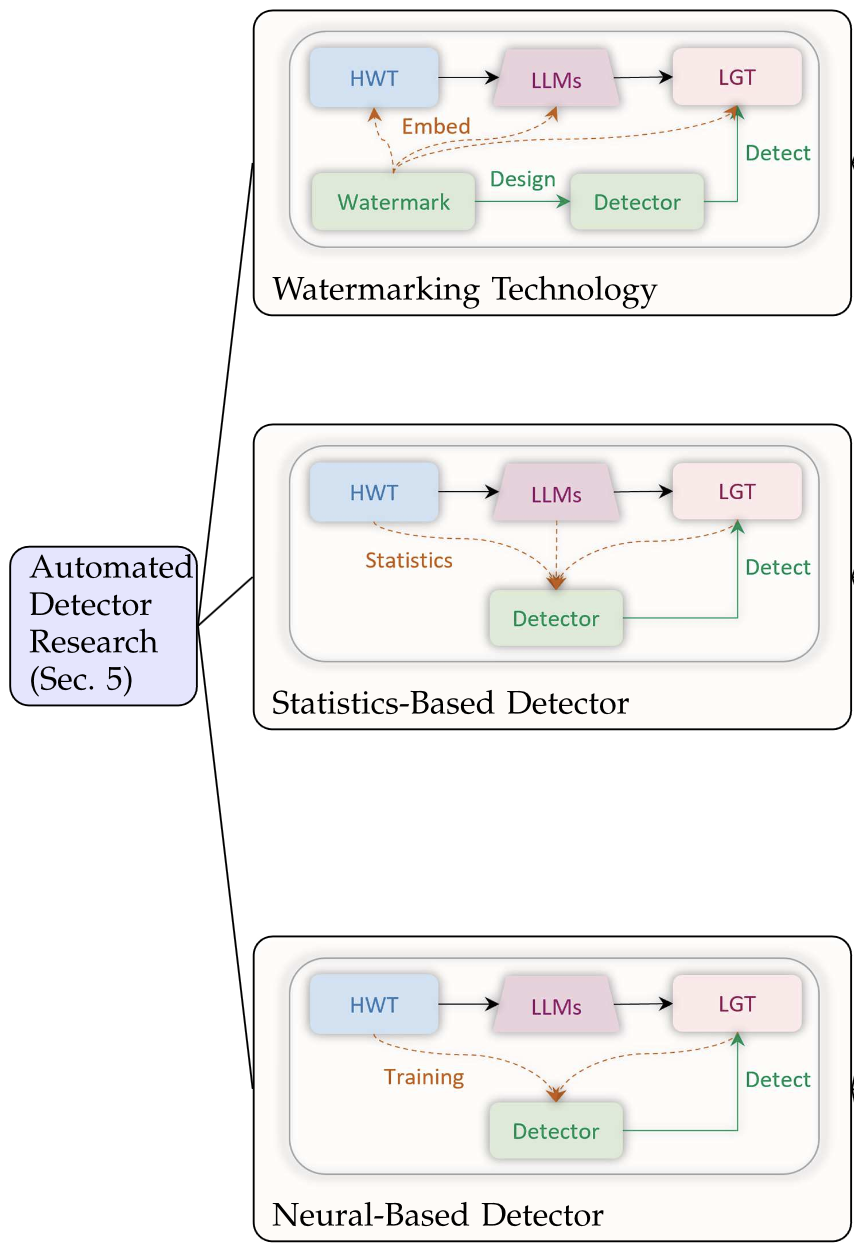
\includegraphics[width=0.8\linewidth]{figure/detector_taxonomy.png}
\end{vbframe}

% ------------------------------------------------------------------------------
% #3
% ------------------------------------------------------------------------------
\begin{vbframe}{What Does a Detector Observe?}

The detector never observes the writing process directly.

\[
\underbrace{\text{model}}_{\text{base + post-training}}
+\underbrace{\text{prompt}}_{\text{task + style + persona}}
+\underbrace{\text{domain}}_{\text{topic + genre}}
+\underbrace{\text{decoding}}_{\text{sampling}}
\longrightarrow x
\]

The detector sees only:

\[
x \longrightarrow D(x)
\]

\begin{center}
\textbf{Therefore, ``AI-likeness'' is confounded with style, topic, genre, prompt, and editing.}
\end{center}

\end{vbframe}


\begin{frame}[plain]
\vfill
\begin{center}
{\LARGE \textbf{Stylometric Differences between Human and AI Text}}
\end{center}
\vfill
\end{frame}

% ------------------------------------------------------------------------------
% #4
% ------------------------------------------------------------------------------
\begin{vbframe}{Classical Roots: Authorship Attribution}

AI-text detection is related to authorship attribution.

\begin{description}
    \item[Authorship attribution]
    Which human author wrote this?
    \[
    P(a_i\mid x)
    \]

    \item[AI-text detection]
    Was this produced by a generative system?
    \[
    P(\text{AI}\mid x)
    \]
\end{description}

Classical stylometry uses stable linguistic habits:

\begin{itemize}
    \item function words,
    \item character and word n-grams,
    \item sentence length,
    \item syntactic patterns,
    \item vocabulary richness.
\end{itemize}

\citebutton{Stamatatos, 2009}{https://doi.org/10.1002/asi.21001}

\end{vbframe}

% ------------------------------------------------------------------------------
% #5
% ------------------------------------------------------------------------------
\begin{vbframe}{Stylometric Features}

Early machine-generated-text detection relied on surface statistics.

\begin{itemize}
    \item function-word density,
    \item phrase and n-gram frequency,
    \item grammatical branching,
    \item constituent length,
    \item fluency and grammaticality features.
\end{itemize}

\begin{center}
\textbf{These features are interpretable, but not necessarily stable across generators.}
\end{center}

\citebutton{Wu et al., 2025, Sec. 5.2.1}{https://direct.mit.edu/coli/article/51/1/275/128271/A-Survey-on-LLM-Generated-Text-Detection}

\end{vbframe}

% ------------------------------------------------------------------------------
% #6
% ------------------------------------------------------------------------------
\begin{vbframe}{Stylometry Is Not Enough}

A feature can separate human and AI text in one dataset and fail in another.

\[
P(f\mid \text{AI},\text{domain A})
\neq
P(f\mid \text{AI},\text{domain B})
\]

\begin{center}
\textbf{The real question is not whether a feature differs, but whether the difference transfers.}
\end{center}

This motivates evaluating across:

\begin{itemize}
    \item prompts,
    \item generator models,
    \item domains,
    \item writing and editing processes.
\end{itemize}

\end{vbframe}

% ------------------------------------------------------------------------------
% #7
% ------------------------------------------------------------------------------
\begin{vbframe}{A Generalization Benchmark}

The benchmark combines:

\begin{itemize}
    \item \textbf{6 prompts:} 0-shot, 3-shot, style, CoT, 1-shot CoT, self-refine,
    \item \textbf{7 LLMs:} Mistral, DeepSeek, Llama, Qwen variants, Solar,
    \item \textbf{4 domains:} abstracts, news, reviews, QA.
\end{itemize}

For every prompt--model--domain condition, a detector is fine-tuned and tested under distribution shifts.

\begin{center}
\textbf{This turns detector evaluation into a controlled transfer problem.}
\end{center}

\citebutton{Xia, Sta\'nczak \& Roth, 2026}{https://aclanthology.org/2026.eacl-long.307/}

\end{vbframe}

% ------------------------------------------------------------------------------
% #8
% ------------------------------------------------------------------------------
\begin{vbframe}{In-Domain Success, Transfer Failure}
\begin{columns}[T]
\begin{column}{0.58\textwidth}


\begin{center}
\textbf{Near-perfect diagonal performance does not imply robust generalization.}

The accuracy of a detector can drop from 99\% to 57\% when the domain changes.

\citebutton{Xia et al., 2026, Fig. 1a}{https://aclanthology.org/2026.eacl-long.307/}

\end{center}

\end{column}

\begin{column}{0.35\textwidth}
\begin{figure}
    \centering
    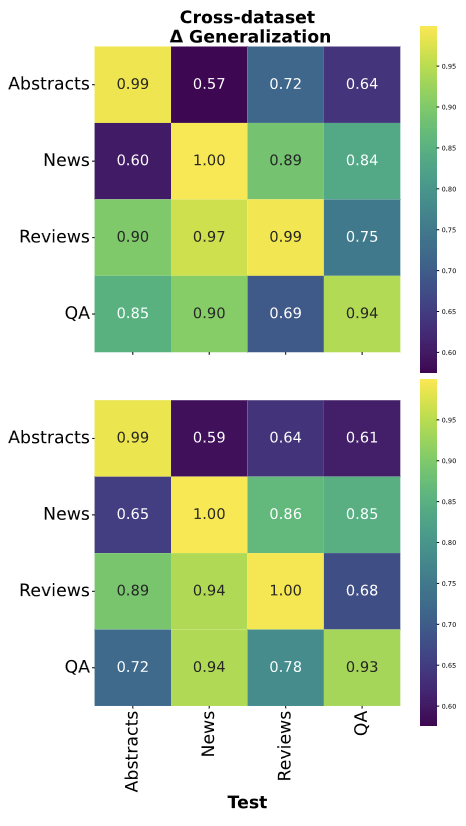
\includegraphics[width=\linewidth]{figure/xia2026_fig1a_generalization_heatmaps.png}
\end{figure}
\end{column}
\end{columns}


\end{vbframe}

% ------------------------------------------------------------------------------
% #9
% ------------------------------------------------------------------------------
\begin{vbframe}{Feature Shifts Explain Some Transfer Gaps}

For a linguistic feature \(f\), define the human--AI feature gap:

\[
f(D)=f(D_{\mathrm{human}})-f(D_{\mathrm{AI}})
\]

The train--test shift is:

\[
\Delta f = f(D_{\mathrm{train}})-f(D_{\mathrm{test}})
\]

Then correlate detector generalization difference (\(\Delta_{\mathrm{gen}}\)), 
the accuracy difference between train and test domain, with feature shifts:

\[
\mathrm{Corr}(f)=
\left|
\mathrm{Pearson}(\Delta_{\mathrm{gen}},\Delta_f)
\right|
\]

\citebutton{Xia et al., 2026, Eq. 4--5}{https://aclanthology.org/2026.eacl-long.307/}

\end{vbframe}

% ------------------------------------------------------------------------------
% #10
% ------------------------------------------------------------------------------
\begin{vbframe}{Robust Linguistic Correlates}

The most robust feature families include (Cross-Prompt, C-P, and Cross-Model, C-M):

\begin{itemize}
    \item pronoun usage, verb tense, active/passive voice,
    \item readability and sentence structure in specific settings.
\end{itemize}
No feature was robust Cross-Domain (C-D)!

\begin{figure}
    \centering
    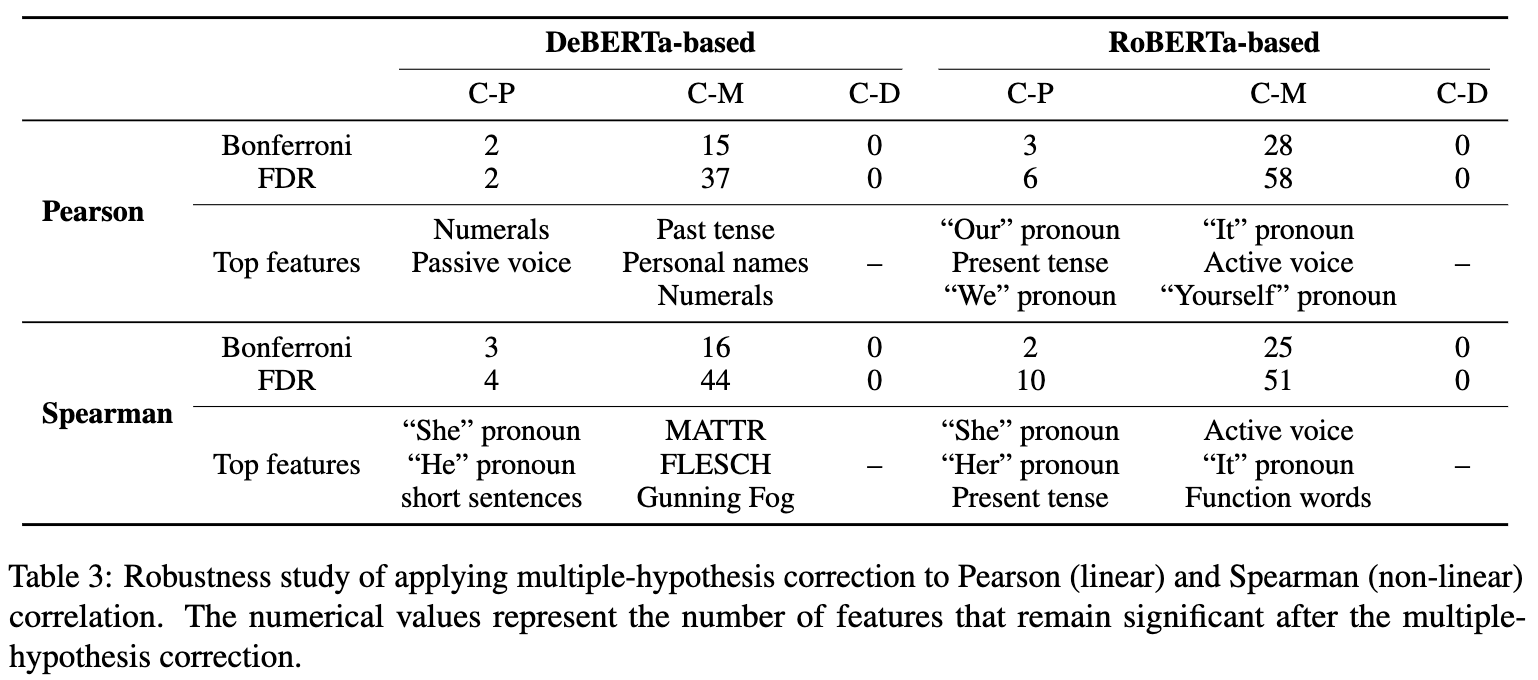
\includegraphics[width=9.8cm]{figure/xia2026_table3_robust_features.png}
\end{figure}

\citebutton{Xia et al., 2026, Table 3}{https://aclanthology.org/2026.eacl-long.307/}

\end{vbframe}

% ------------------------------------------------------------------------------
% #11
% ------------------------------------------------------------------------------
\begin{vbframe}{Human--AI Feature Differences}

    \begin{columns}[T]
\begin{column}{0.40\textwidth}
In this benchmark, AI text often uses less of some features than human text, e.g. passive voice, past tense, and the pronoun ``it''.

\citebutton{Xia et al., 2026, Fig. 4}{https://aclanthology.org/2026.eacl-long.307/}
\end{column}

\begin{column}{0.58\textwidth}
\begin{figure}
    \centering
    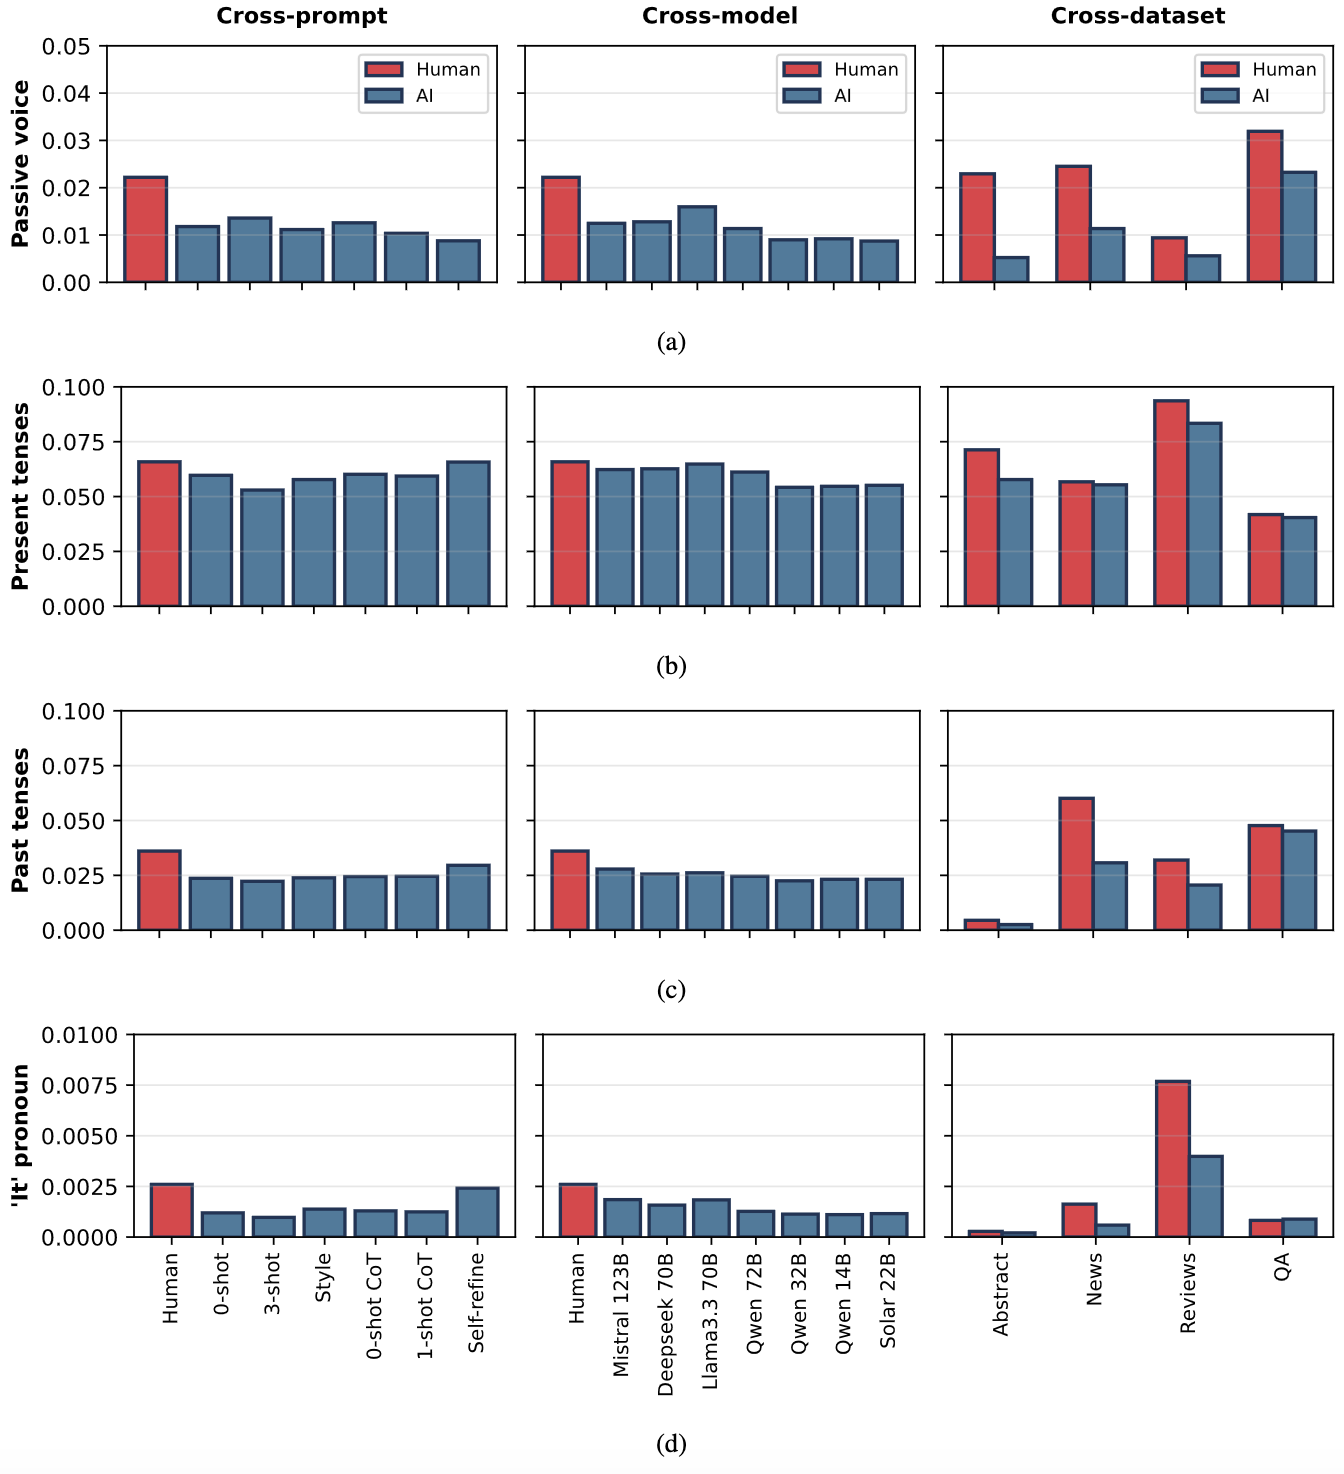
\includegraphics[width=\linewidth]{figure/xia2026_fig4_feature_distributions.png}
\end{figure}
\end{column}
\end{columns}
%\begin{center}
%\textbf{But the key point is stability of the gap, not the feature alone.}
%\end{center}
\end{vbframe}

% ------------------------------------------------------------------------------
% #12
% ------------------------------------------------------------------------------
%\begin{vbframe}{Aggregation Can Hide Mechanisms}
%\begin{figure}
%    \centering
%    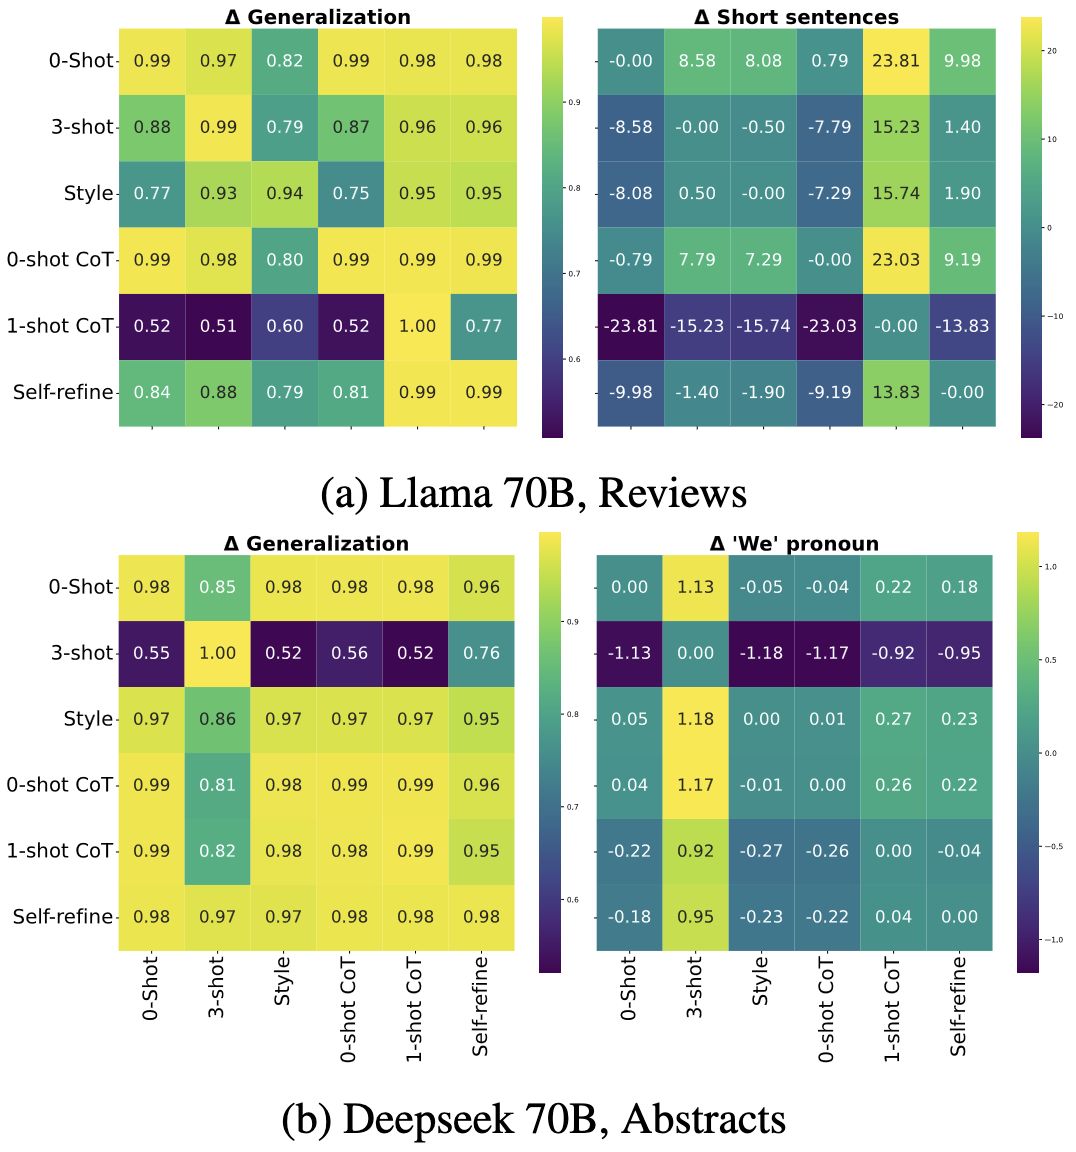
\includegraphics[width=5cm]{figure/xia2026_fig2_local_prompt_effects.png}
%\end{figure}
%Overall correlations can look weak even when a specific model--domain setting has a strong linguistic dependency.
%\begin{center}
%\textbf{Explanations may be local to model, prompt, and domain.}
%\end{center}
%\citebutton{Xia et al., 2026, Fig. 2}{https://aclanthology.org/2026.eacl-long.307/}
%\end{vbframe}


\begin{frame}[plain]
\vfill
\begin{center}
{\LARGE \textbf{Likelihood-Based and Unsupervised Detectors}}
\end{center}
\vfill
\end{frame}

% ------------------------------------------------------------------------------
% #13
% ------------------------------------------------------------------------------
\begin{vbframe}{Likelihood and Perplexity}

For an autoregressive language model \(M\):

\[
P_M(x_{1:T})=\prod_{t=1}^{T}P_M(x_t\mid x_{<t})
\]

Average log-likelihood:

\[
\frac{1}{T}\sum_{t=1}^{T}\log P_M(x_t\mid x_{<t})
\]

Perplexity:

\[
\mathrm{PPL}_M(x)=
\exp\left(-\frac{1}{T}\sum_{t=1}^{T}
\log P_M(x_t\mid x_{<t})\right)
\]

\begin{center}
\textbf{High perplexity = high average surprisal = low average log-likelihood.}
\end{center}

\end{vbframe}

% ------------------------------------------------------------------------------
% #14
% ------------------------------------------------------------------------------
\begin{vbframe}{GLTR: Token Ranks as Visual Evidence}

\begin{figure}
    \centering
    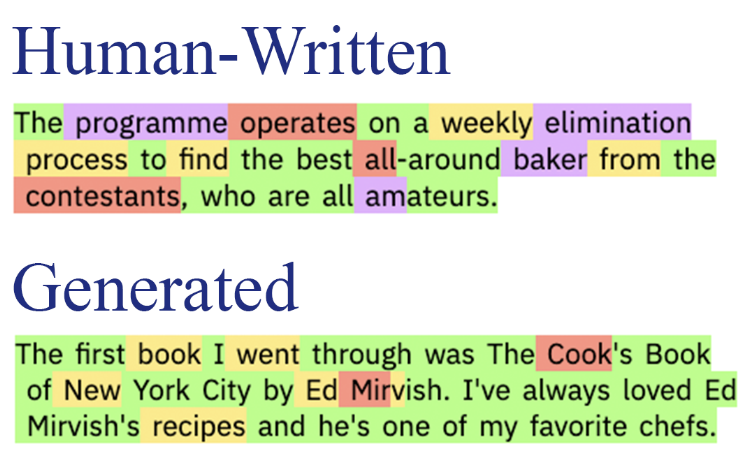
\includegraphics[width=5cm]{figure/gltr2019_fig1_token_rank_highlighting.png}
\citebutton{Gehrmann et al., 2019, Fig. 1}{https://aclanthology.org/P19-3019/}
\end{figure}


GLTR (Giant Language model Test Room) highlights each token according to its rank under a language model.

\begin{center}
\textbf{Generated text often overuses high-probability tokens.}
\end{center}


\end{vbframe}

% ------------------------------------------------------------------------------
% #15
% ------------------------------------------------------------------------------
\begin{vbframe}{Perplexity Detectors Use a Scoring Model}

A detector can score ChatGPT text using another model, e.g. GPT-2.

\[
\mathrm{PPL}_{\mathrm{GPT\text{-}2}}(x)
\]

%This is not the same as asking for the probability under the true generator.
%\begin{center}
%\textbf{Perplexity is always relative to the scoring model.}
%\end{center}

Useful distinction:

\begin{itemize}
    \item generator likelihood: \(P_G(x)\),
    \item surrogate likelihood: \(P_S(x)\).
\end{itemize}

\citebutton{Vasilatos et al., 2023}{https://arxiv.org/abs/2305.18226}

\end{vbframe}

% ------------------------------------------------------------------------------
% #16
% ------------------------------------------------------------------------------
\begin{vbframe}{DetectGPT: Probability Curvature}

\begin{figure}
    \centering
    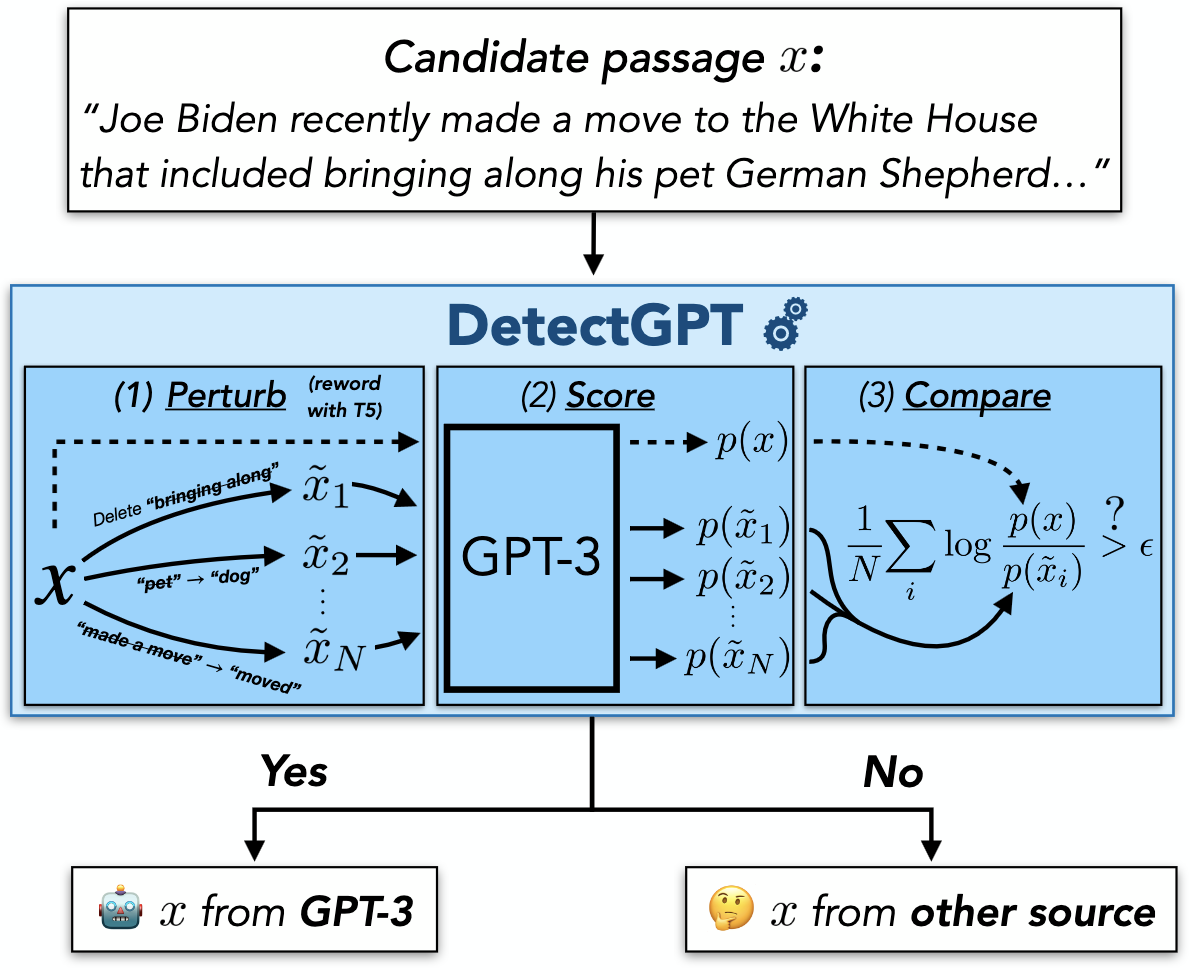
\includegraphics[width=5cm]{figure/detectgpt2023_fig1_probability_curvature.png}
\end{figure}

DetectGPT asks whether the original text is more likely than nearby paraphrases. \citebutton{Mitchell et al., 2023, Fig. 1}{https://proceedings.mlr.press/v202/mitchell23a.html}

\[
d(x)=\log p_\theta(x)-
\mathbb{E}_{\tilde{x}\sim q(\cdot\mid x)}
\left[\log p_\theta(\tilde{x})\right]
\]


\end{vbframe}

% ------------------------------------------------------------------------------
% #17
% ------------------------------------------------------------------------------
\begin{vbframe}{Why ``Curvature''?}

Machine-generated text may lie near local maxima of the model's log-probability surface.

\[
\log p_\theta(x)
>
\mathbb{E}_{\tilde{x}}[\log p_\theta(\tilde{x})]
\]

Text is discrete, so curvature is estimated through perturbations rather than derivatives. 
\citebutton{Mitchell et al., 2023}{https://proceedings.mlr.press/v202/mitchell23a.html}

\begin{figure}
    \centering
    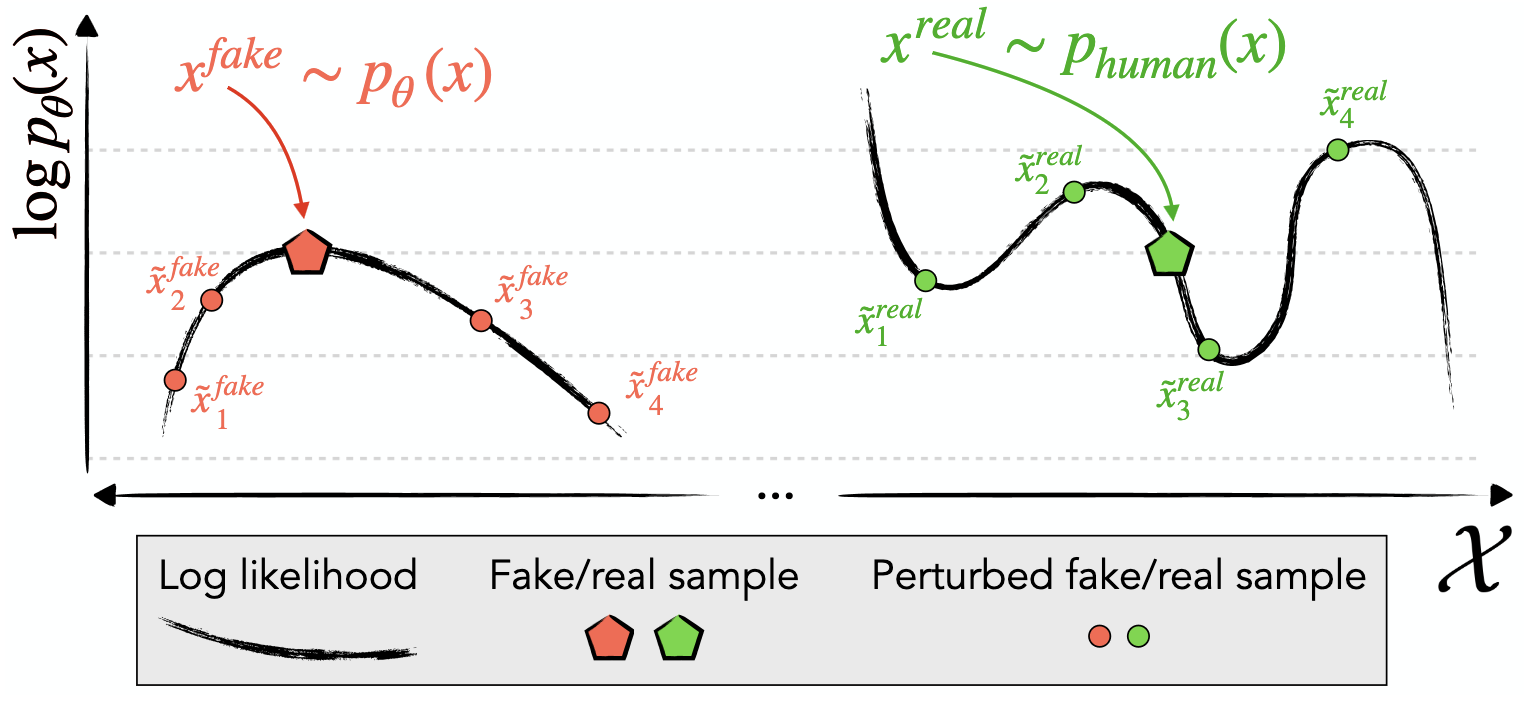
\includegraphics[width=9cm]{figure/detectgpt2023_fig2_probability_curvature.png}
\end{figure}

%\begin{center}
%\textbf{Same likelihood, different local geometry.}
%\end{center}

%\citebutton{Mitchell et al., 2023, Algorithm 1}{https://proceedings.mlr.press/v202/mitchell23a.html}

\end{vbframe}

% ------------------------------------------------------------------------------
% #20
% ------------------------------------------------------------------------------
\begin{vbframe}{Intrinsic Dimension}

Another signal: the geometry of contextual token embeddings.

\[
\{e_1,\ldots,e_T\}\subset \mathbb{R}^d
\]

The text is represented as a point cloud. Its intrinsic dimension is estimated using persistent homology / MST scaling.

\begin{figure}
    \centering
    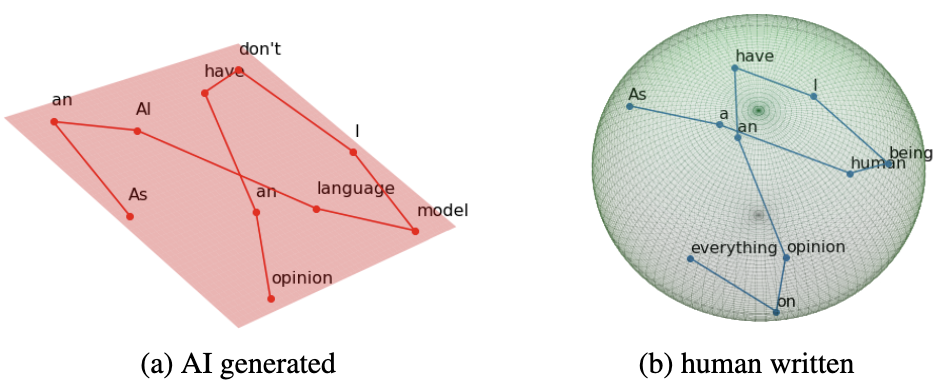
\includegraphics[width=9.5cm]{figure/tulchinskii2023_dimension_distribution.png}
\end{figure}

\begin{center}
\textbf{Machine text may explore fewer independent representational directions.}
\end{center}

\citebutton{Tulchinskii et al., 2023}{https://arxiv.org/abs/2306.04723}

\end{vbframe}



\begin{frame}[plain]
\vfill
\begin{center}
{\LARGE \textbf{Trained Detectors}}
\end{center}
\vfill
\end{frame}

% ------------------------------------------------------------------------------
% #21
% ------------------------------------------------------------------------------
\begin{vbframe}{Trained Detectors}

Modern strong detectors are usually supervised classifiers.

\[
x
\xrightarrow{\text{encoder / backbone}}
h(x)
\xrightarrow{\text{classification head}}
\hat y
\]

RoBERTa/BERT-style detectors often perform very well in-domain, but can overfit to model and domain distributions.

\begin{center}
\textbf{In practice, the training distribution is often more important than the architecture.}
\end{center}

\citebutton{Wu et al., 2025, Sec. 5.3}{https://direct.mit.edu/coli/article/51/1/275/128271/A-Survey-on-LLM-Generated-Text-Detection}

\end{vbframe}

% ------------------------------------------------------------------------------
% #22
% ------------------------------------------------------------------------------
\begin{vbframe}{Where Does Training Data Come From?}

A supervised detector needs labeled examples:

\[
\{(x_i,y_i)\}_{i=1}^{N}
\]

But the hard part is not just scale.

\begin{center}
\textbf{Human and AI examples must be matched for topic, genre, length, and task.}
\end{center}

Otherwise, the classifier may learn:

\[
\text{news vs essays}
\quad\text{instead of}\quad
\text{human vs AI}.
\]

\end{vbframe}

% ------------------------------------------------------------------------------
% #23
% ------------------------------------------------------------------------------
\begin{vbframe}{Pangram: Synthetic Mirrors}

\begin{figure}
    \centering
    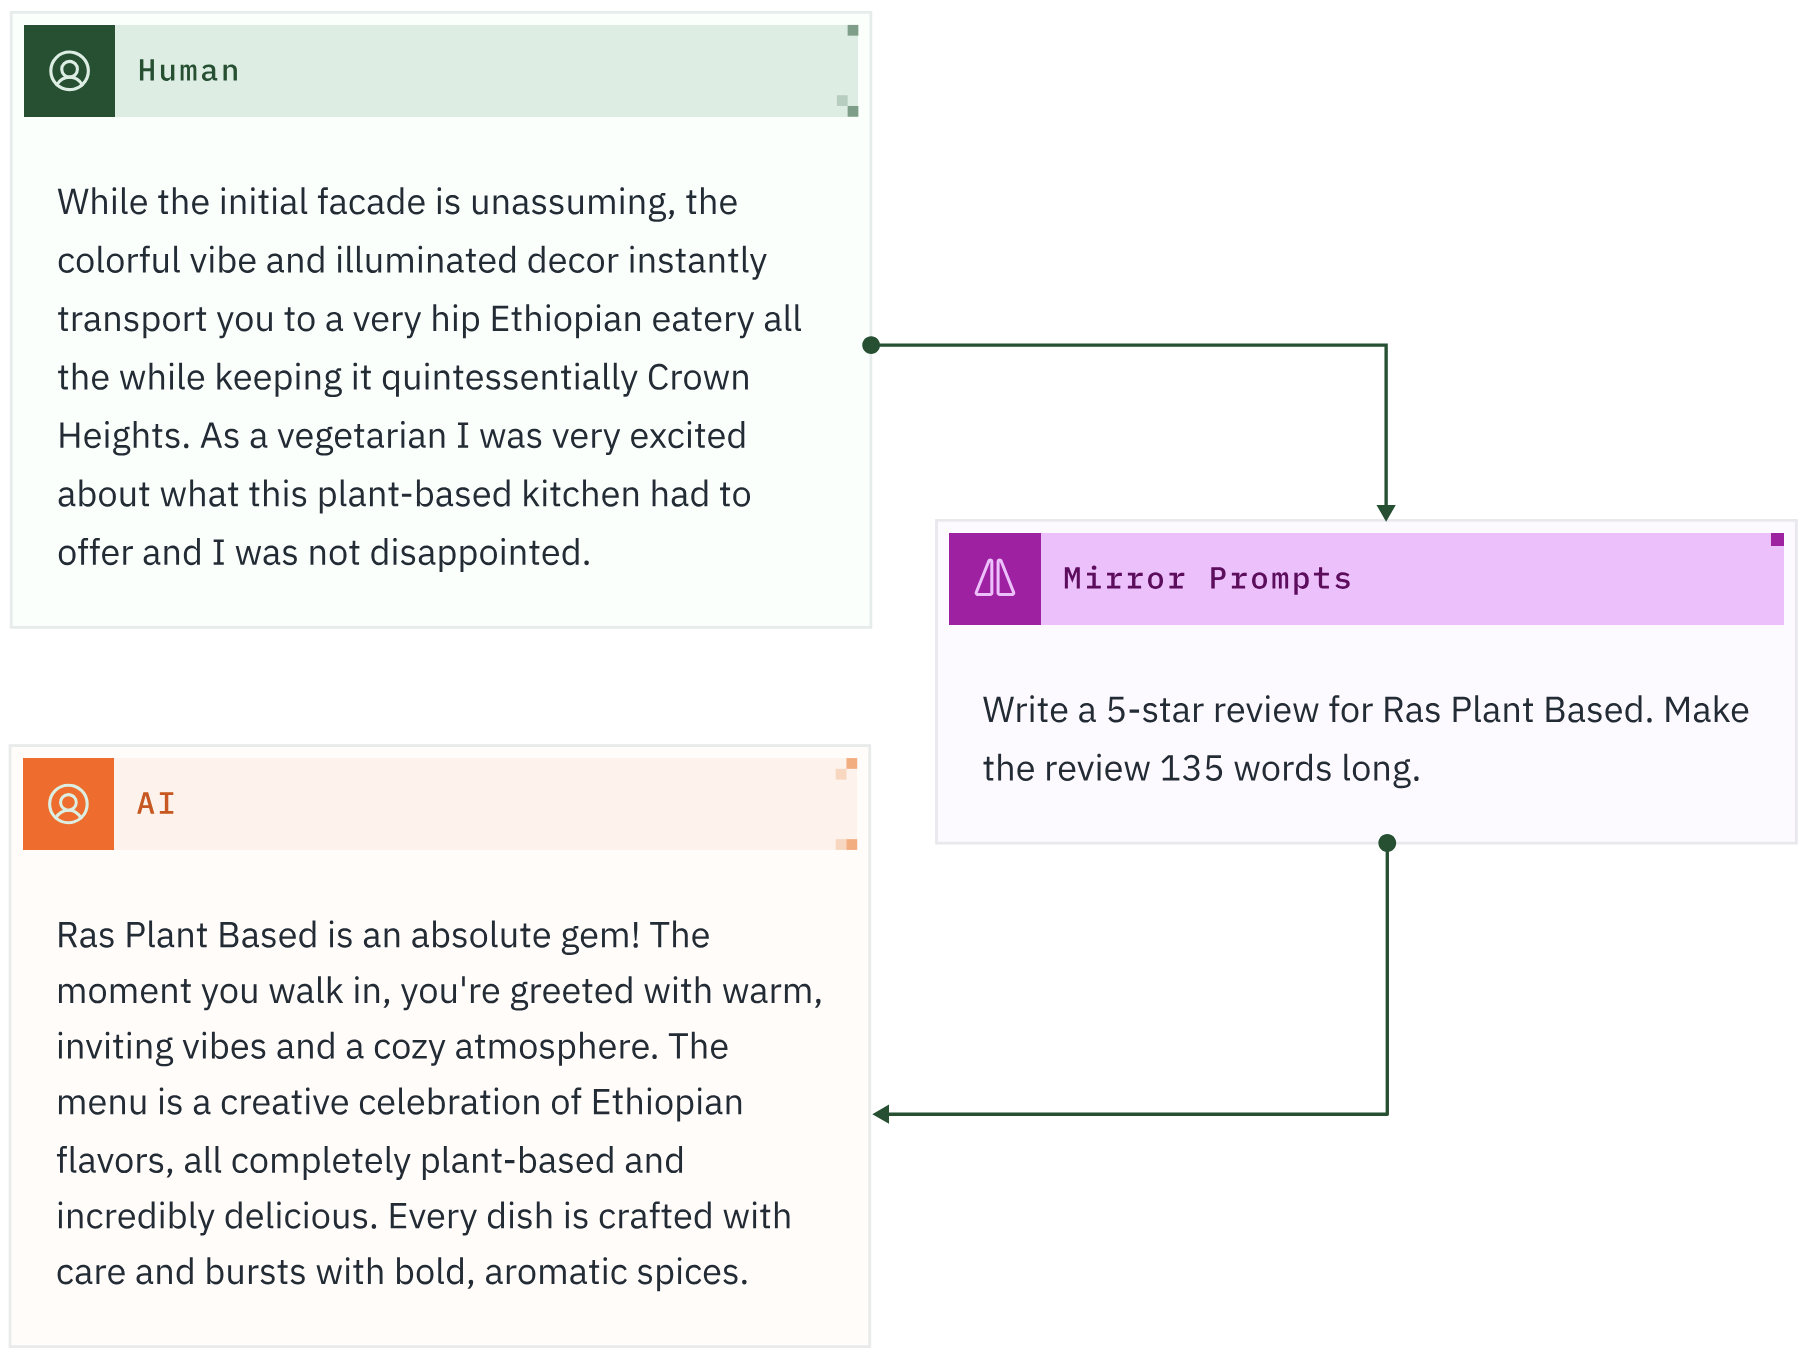
\includegraphics[width=7cm]{figure/pangram_synthetic_mirrors_fig5.png}\citebutton{Pangram, How AI Detection Works}{https://www.pangram.com/research/how-it-works}
\end{figure}

Pangram describes generating AI examples that mirror human documents in topic, genre, length, and style.

\[
\text{human text}
\longrightarrow
\text{matched synthetic mirror}
\]

\end{vbframe}

% ------------------------------------------------------------------------------
% #24
% ------------------------------------------------------------------------------
\begin{vbframe}{Pangram: Hard-Negative Mining}


\begin{columns}[T]

\begin{column}{0.40\textwidth}
\begin{figure}
    \centering
    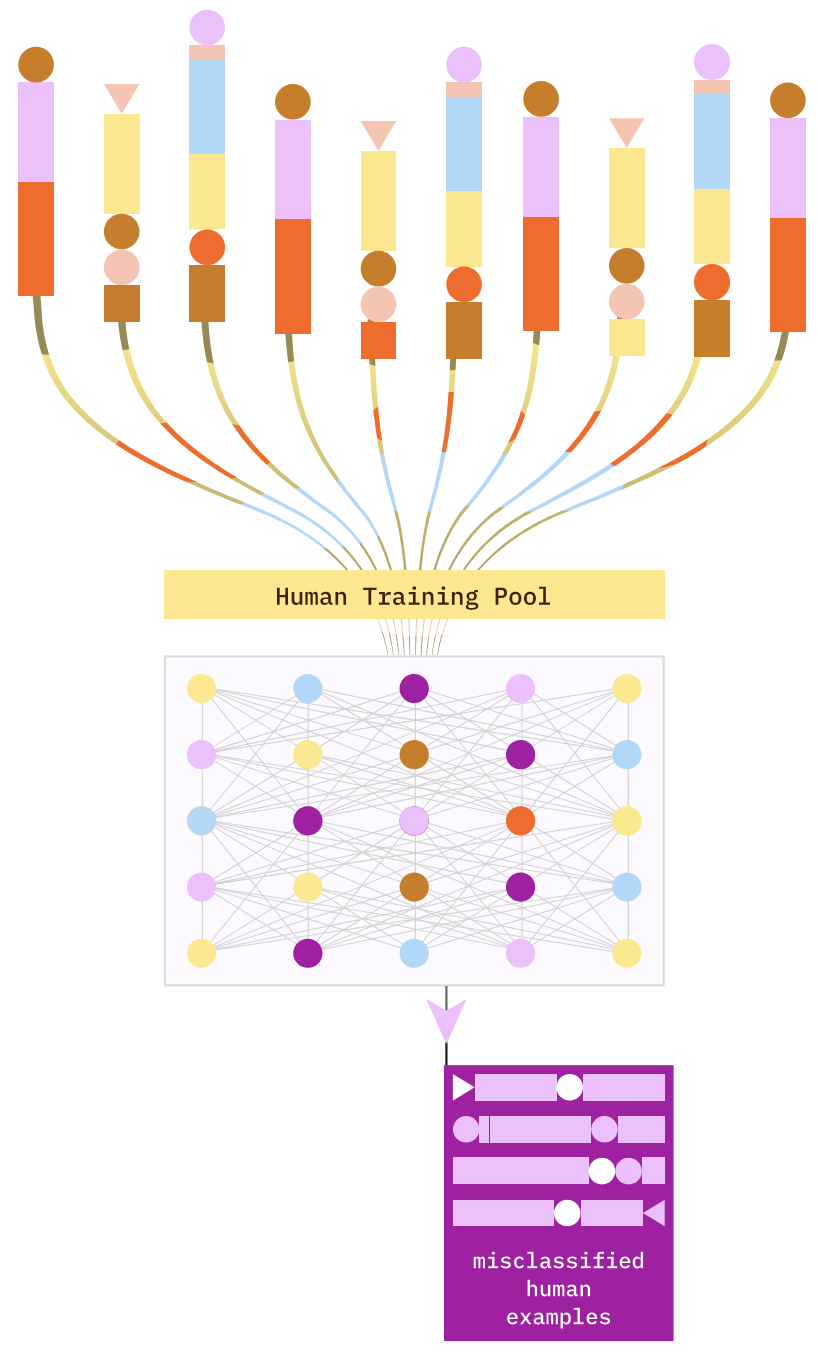
\includegraphics[width=\linewidth]{figure/pangram_hard_negative_mining_fig4.png}
\end{figure}
\end{column}

\begin{column}{0.58\textwidth}
The detector is run on human corpora to find false positives.
\[
\text{hard human examples}
\rightarrow
\text{training set}
\]
\[
\rightarrow
\text{retrain}
\]
\citebutton{Pangram, How AI Detection Works}{https://www.pangram.com/research/how-it-works}
\end{column}

\end{columns}




%\begin{center}
%\textbf{This is good engineering, but it also shows that errors are distribution-dependent.}
%\end{center}
\end{vbframe}

% ------------------------------------------------------------------------------
% #25
% ------------------------------------------------------------------------------
\begin{vbframe}{Pangram 4}

\begin{figure}
    \centering
    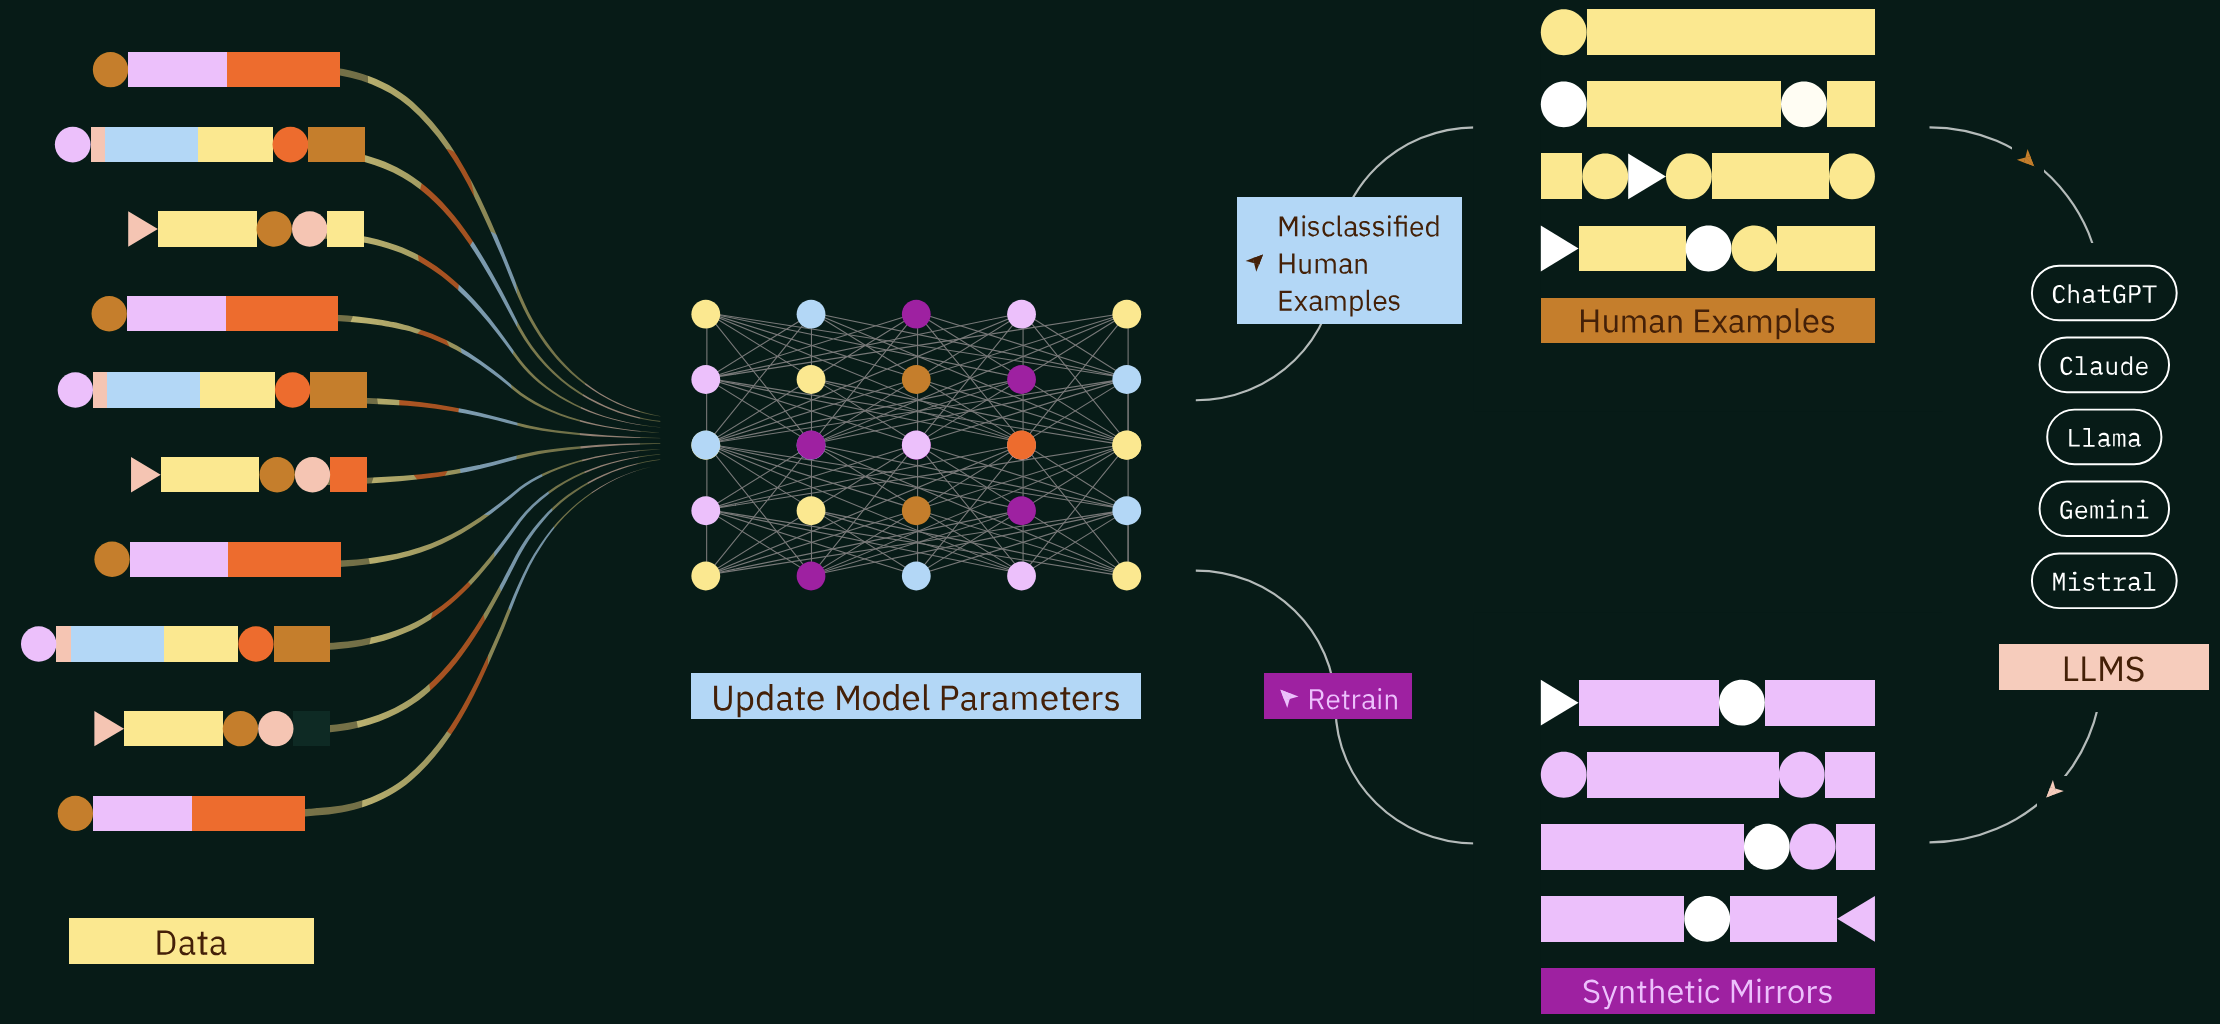
\includegraphics[width=8cm]{figure/pangram4_2026_architecture_fig1.png}
\end{figure}

Pangram 4 reports:

\begin{itemize}
    \item sparse mixture-of-experts backbone,
    \item document-level AI-assistance score,
    \item token-level provenance,
    \item mixed-authorship and humanizer heads.
\end{itemize}

\citebutton{Pangram 4 Technical Report, 2026, Fig. 1}{https://arxiv.org/abs/2607.27183}

\end{vbframe}

% ------------------------------------------------------------------------------
% #26
% ------------------------------------------------------------------------------
\begin{vbframe}{GPTZero: Commercial Detector Pipeline}

\begin{figure}
    \centering
    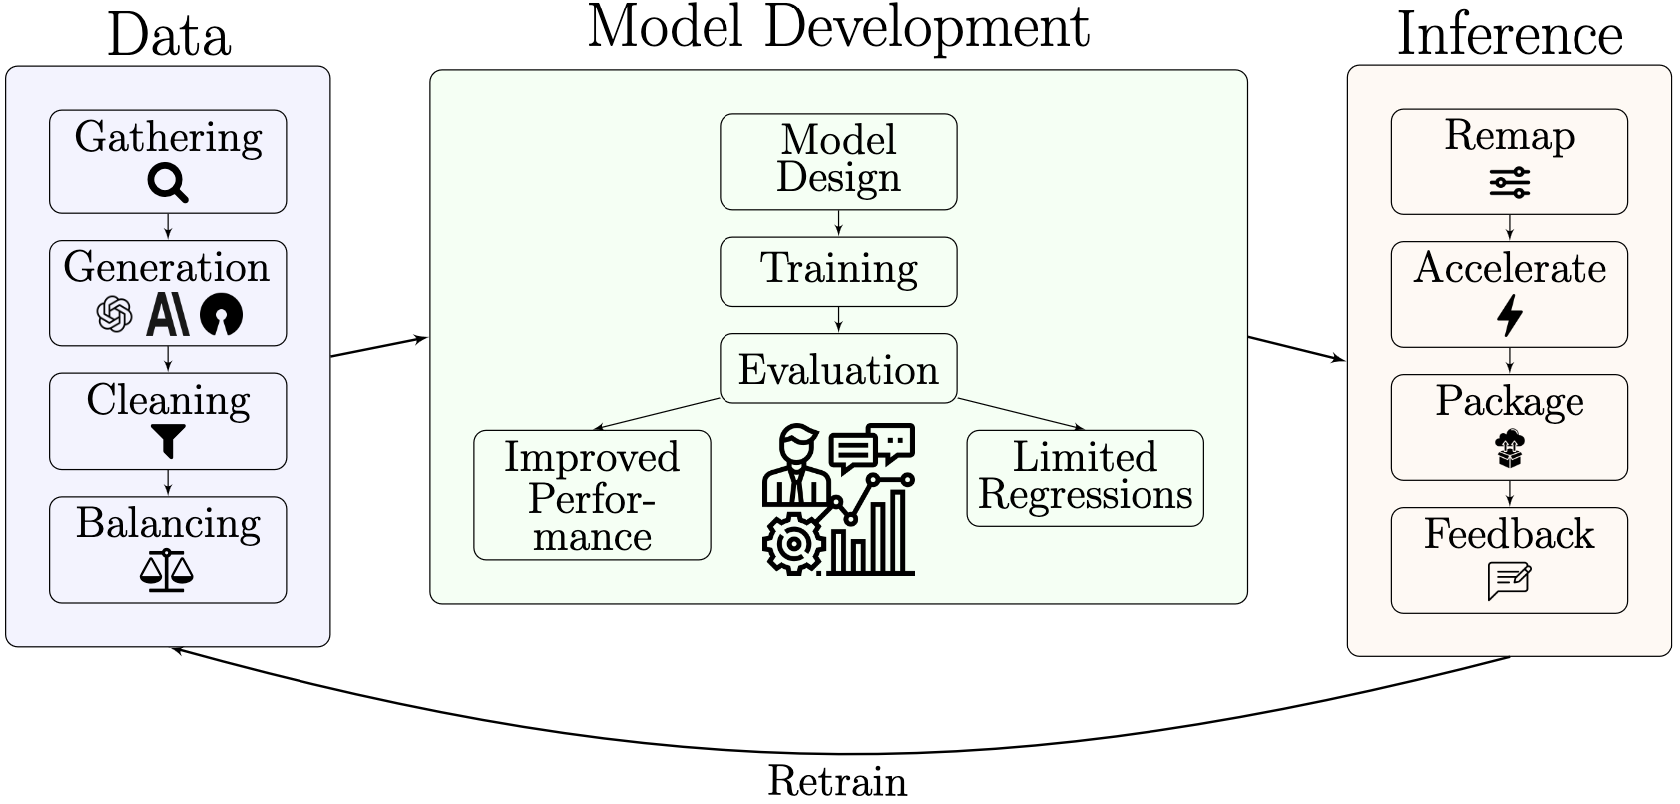
\includegraphics[width=6cm]{figure/gptzero2026_pipeline_fig1.png}
\end{figure}

GPTZero describes a supervised hierarchical detector for:

\begin{itemize}
    \item human,
    \item AI,
    \item mixed,
    \item polished,
    \item paraphrased text.
\end{itemize}

\citebutton{Adam et al., 2026, Fig. 1}{https://arxiv.org/abs/2602.13042}

\end{vbframe}

% ------------------------------------------------------------------------------
% #27
% ------------------------------------------------------------------------------
\begin{vbframe}{Commercial Metrics: A Caution}

Vendor-reported metrics are tied to the vendor's evaluation distribution.

\[
\mathrm{FPR}_{\mathrm{vendor}}
\neq
\mathrm{FPR}_{\mathrm{your\ population}}
\]

Ask:

\begin{itemize}
    \item Which domains and authors?
    \item Which LLMs and model versions?
    \item Which prompts and editing conditions?
    \item Which detector version?
    \item Independent or vendor-authored evaluation?
\end{itemize}

\begin{center}
\textbf{A metric is not an intrinsic property of a detector.}
\end{center}

\end{vbframe}

% ------------------------------------------------------------------------------
% #28
% ------------------------------------------------------------------------------
\begin{vbframe}{What Does ``99\% AI'' Mean?}

A displayed number may mean different things:

\begin{itemize}
    \item classifier score,
    \item calibrated class probability,
    \item percentage of qualifying text,
    \item confidence category,
    \item posterior probability in a forensic context.
\end{itemize}

Calibration requires:

\[
P(Y=1\mid \hat p=p)=p
\]

\begin{center}
\textbf{A score in \([0,1]\) is not automatically a probability.}
\end{center}

\end{vbframe}

% ------------------------------------------------------------------------------
% #29
% ------------------------------------------------------------------------------
\begin{vbframe}{Base Rates Matter}

Even excellent detectors can produce many false accusations if the base rate is low.

\[
P(\mathrm{AI}\mid +)=
\frac{P(+\mid \mathrm{AI})P(\mathrm{AI})}
{P(+\mid \mathrm{AI})P(\mathrm{AI})+P(+\mid H)P(H)}
\]

Example:

\[
\mathrm{TPR}=0.99,
\quad
\mathrm{FPR}=0.01,
\quad
P(\mathrm{AI})=0.01
\]

\[
P(\mathrm{AI}\mid +)=0.5
\]

\begin{center}
\textbf{The same detector can imply different posteriors in different populations.}
\end{center}

\end{vbframe}

% ------------------------------------------------------------------------------
% #30
% ------------------------------------------------------------------------------
\begin{vbframe}{RAID: Robust Evaluation}

\begin{figure}
    \centering
    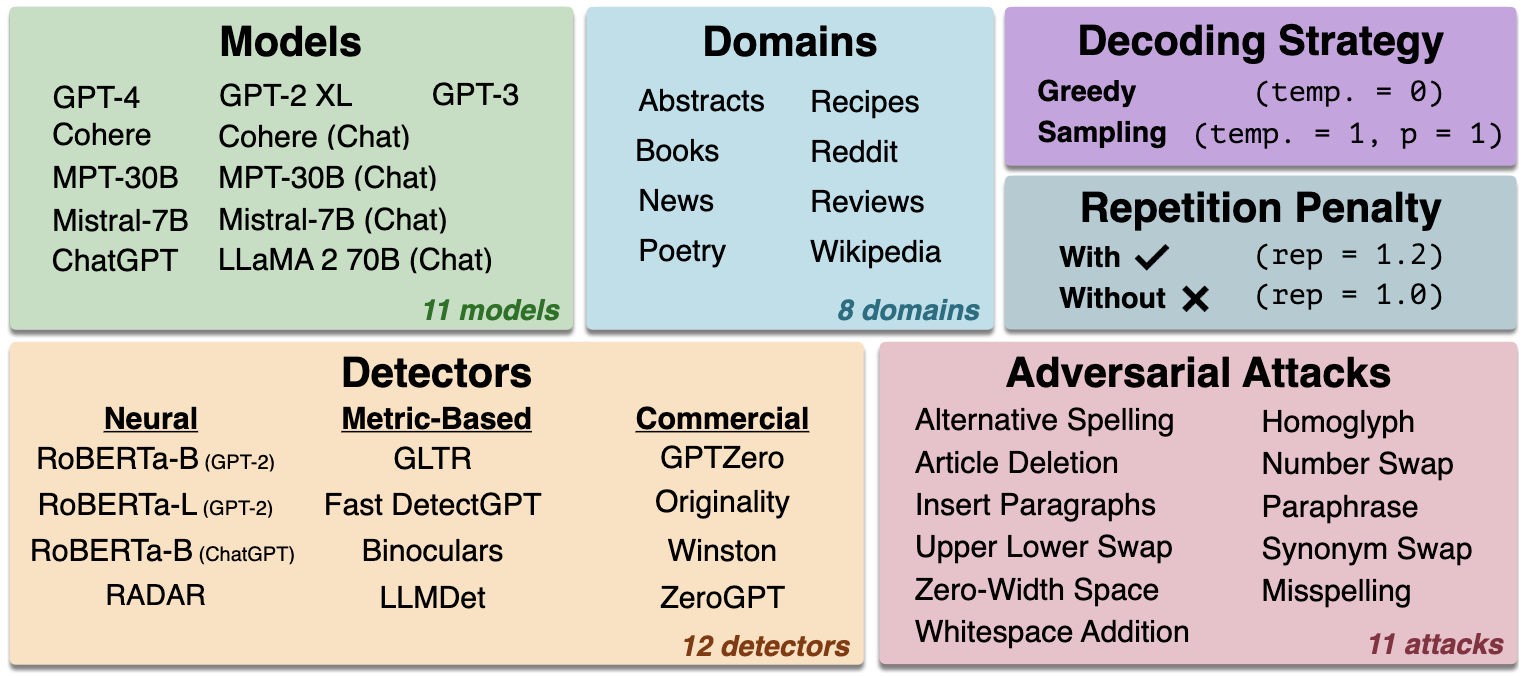
\includegraphics[width=8cm]{figure/raid2024_fig2_benchmark_design.png}
\end{figure}

RAID evaluates detectors across: \citebutton{Dugan et al., 2024, Fig. 2}{https://aclanthology.org/2024.acl-long.674/}

\begin{itemize}
    \item generators,
    \item domains,
    \item decoding strategies,
    \item adversarial attacks.
\end{itemize}

\begin{center}
\textbf{Condition performance on the test distribution.}
\end{center}
\end{vbframe}

% ------------------------------------------------------------------------------
% #31
% ------------------------------------------------------------------------------
\begin{vbframe}{Mixed Authorship and Editing}

\begin{figure}
    \centering
    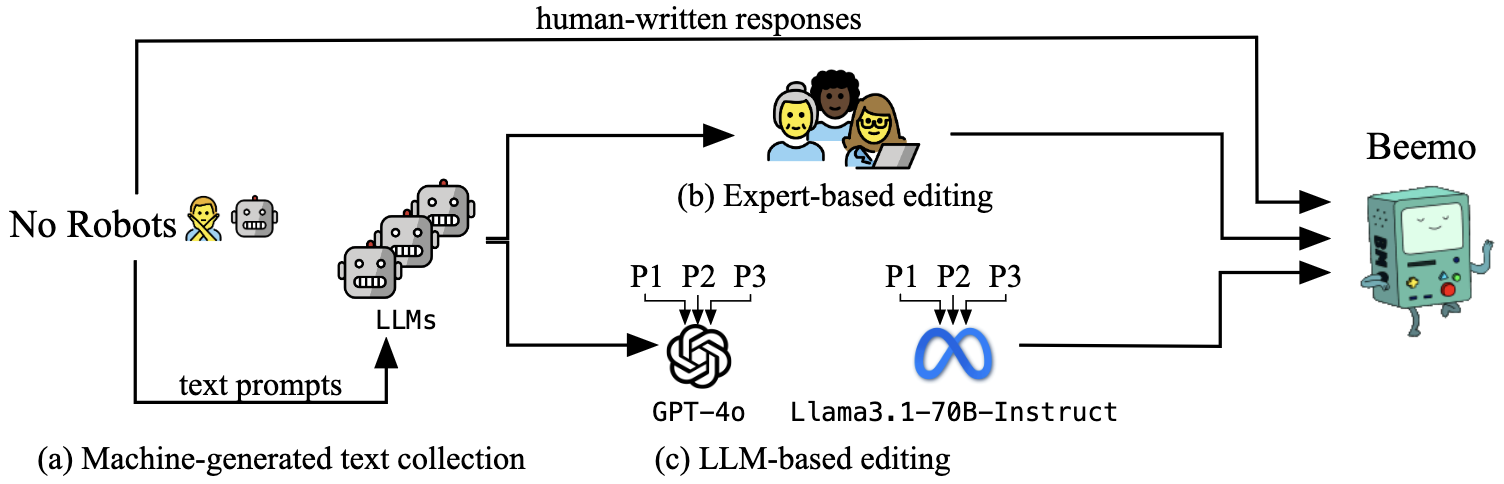
\includegraphics[width=10.5cm]{figure/beemo2025_fig1_editing_pipeline.png}
\end{figure}

Real texts often lie on a continuum:

\[
\text{human}
\rightarrow
\text{AI-polished human}
\rightarrow
\text{mixed}
\rightarrow
\text{human-edited AI}
\rightarrow
\text{AI}
\]

\begin{center}
\textbf{Binary labels become scientifically questionable.}
\end{center}

\citebutton{Artemova et al., 2025, Fig. 1 / Table 4}{https://aclanthology.org/2025.naacl-long.357/}

\end{vbframe}

% ------------------------------------------------------------------------------
% #32
% ------------------------------------------------------------------------------
\begin{vbframe}{Prompt and Style Attacks}

Changing only the prompt can change detectability.

\[
P(x\mid \text{LLM},\text{default prompt})
\neq
P(x\mid \text{LLM},\text{style prompt})
\]

Examples:

\begin{itemize}
    \item write like Shakespeare,
    \item imitate a human example,
    \item use self-refinement to sound more human,
    \item avoid assistant-like phrasing.
\end{itemize}

\begin{center}
\textbf{The same generator can produce different detector signals.}
\end{center}

\citebutton{Zhang et al., 2024}{https://aclanthology.org/2024.findings-naacl.29/}

\end{vbframe}

% ------------------------------------------------------------------------------
% #33
% ------------------------------------------------------------------------------
\begin{vbframe}{Sadasivan et al.: A Theoretical Limit}

Sadasivan et al. show that passive detection becomes impossible as machine text approaches the human distribution.

\[
\mathrm{AUROC}(D)
\leq
\frac{1}{2}
+
\mathrm{TV}(P_{\mathrm{AI}},P_{\mathrm{human}})
-
\frac{1}{2}\mathrm{TV}(P_{\mathrm{AI}},P_{\mathrm{human}})^2
\]

\begin{center}
\textbf{If total variation (distributional difference) between the AI distribution $P_{\mathrm{AI}}$ and the human distribution $P_{\mathrm{human}}$ goes to zero, no passive detector can do much better than chance.}
\end{center}

\citebutton{Sadasivan et al., 2023}{https://arxiv.org/abs/2303.11156}

\end{vbframe}

% ------------------------------------------------------------------------------
% #34
% ------------------------------------------------------------------------------
\begin{vbframe}{But: Better Does Not Mean More Human-Like}

The Sadasivan argument is valid as a mathematical statement about converging distributions.

But the empirical premise is not guaranteed:

\[
\text{more capable model}
\not\Rightarrow
P_{\mathrm{AI}} \to P_{\mathrm{human}}
\]

New model versions can become:

\begin{itemize}
    \item more instruction-following,
    \item more aligned to assistant conventions,
    \item more formulaic in product settings,
    \item more responsive to style constraints.
\end{itemize}

\begin{center}
\textbf{Model improvement and human-likeness are different dimensions.}
\end{center}

\end{vbframe}

% ------------------------------------------------------------------------------
% #35
% ------------------------------------------------------------------------------
\begin{vbframe}{Base Models Look Human to Detectors}

\begin{figure}
    \centering
    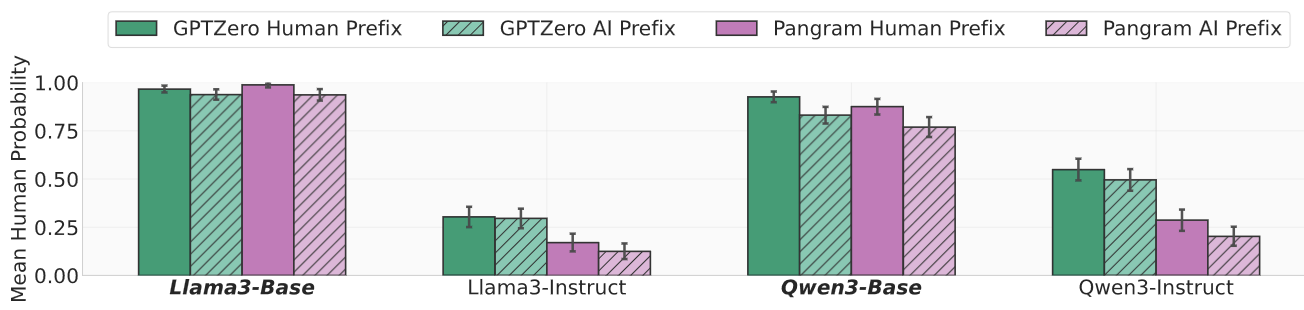
\includegraphics[width=10.4cm]{figure/xu2026_base_models_look_human_fig1.png}
\end{figure}

Xu et al. find that base-model outputs can look more human to detectors than instruction-tuned outputs.

\begin{center}
\textbf{Detectors may track post-training or assistant-style artifacts, not only machine generation.}
\end{center}

\citebutton{Xu et al., 2026, Fig. 1}{https://arxiv.org/abs/2605.19516}

\end{vbframe}


\begin{frame}[plain]
\vfill
\begin{center}
{\LARGE \textbf{Watermarking}}
\end{center}
\vfill
\end{frame}

% ------------------------------------------------------------------------------
% #36
% ------------------------------------------------------------------------------
\begin{vbframe}{From Passive Detection to Watermarking}

Passive detection asks:

\[
\text{Does this text statistically look AI-generated?}
\]

Watermarking asks:

\[
\text{Does this text contain a signal inserted by a known generator?}
\]

Watermarking requires access to generation or deployment.

\citebutton{Wu et al., 2025, Sec. 5.1}{https://direct.mit.edu/coli/article/51/1/275/128271/A-Survey-on-LLM-Generated-Text-Detection}

\end{vbframe}

% ------------------------------------------------------------------------------
% #37
% ------------------------------------------------------------------------------
\begin{vbframe}{Green-Red-List Watermarking}


\begin{columns}[T]
\begin{column}{0.40\textwidth}
At each generation step:

\begin{enumerate}
    \item use a secret key and context to split vocabulary into green/red tokens,
    \item add a logit bias \(\delta\) to green tokens,
    \item sample normally,
    \item later count green tokens.
\end{enumerate}

\citebutton{Kirchenbauer et al., 2023}{https://proceedings.mlr.press/v202/kirchenbauer23a.html}

\end{column}

\begin{column}{0.58\textwidth}

\begin{figure}
    \centering
    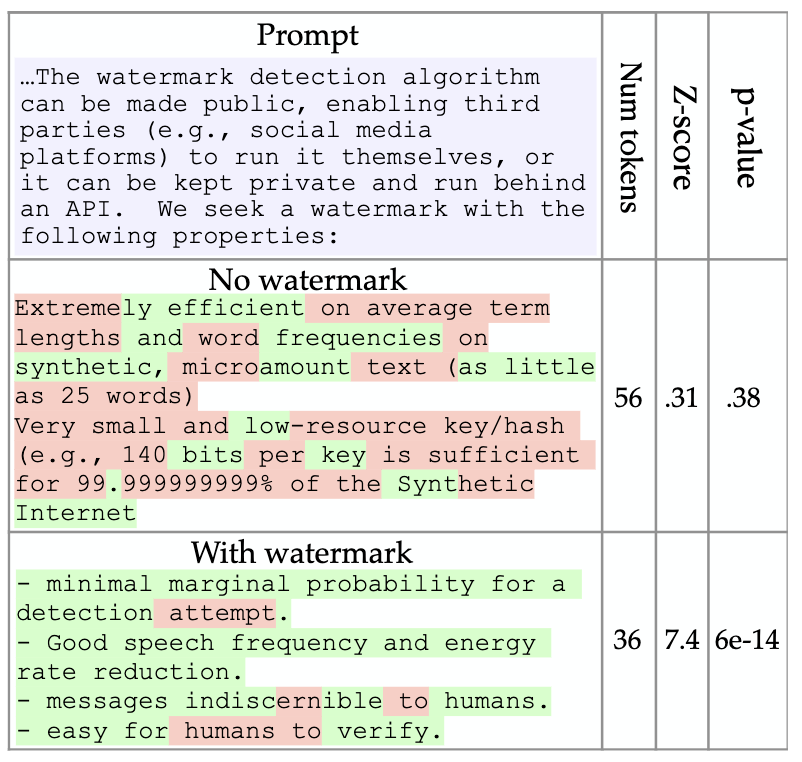
\includegraphics[width=\linewidth]{figure/kirchenbauer2023_greenlist_example.png}
\end{figure}

\end{column}
\end{columns}



\end{vbframe}


\begin{vbframe}{A Simplified Algorithm}

\begin{figure}
    \centering
    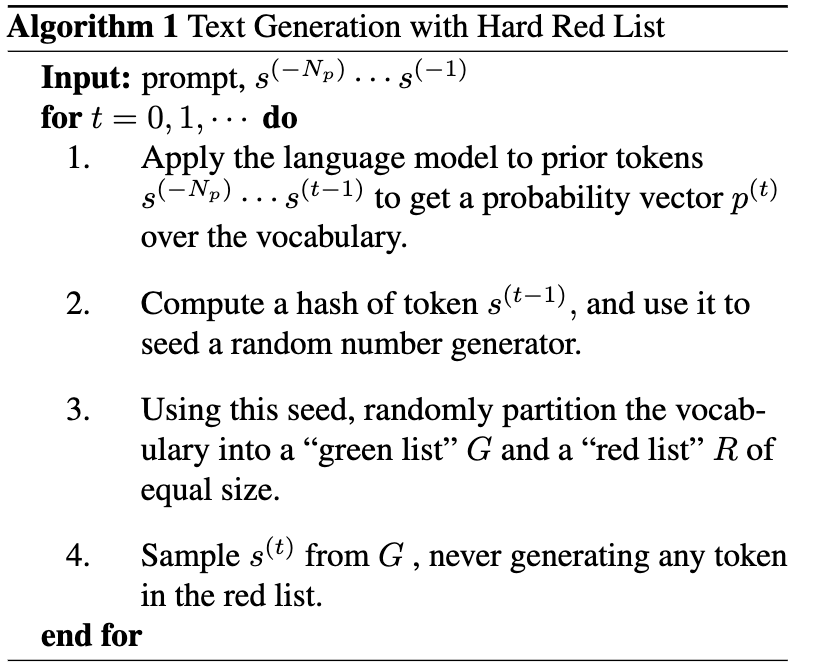
\includegraphics[width=5.5cm]{figure/kirchenbauer2023_simplified.png}
\end{figure}

\end{vbframe}


\begin{vbframe}{The Actual Algorithm}

\begin{figure}
    \centering
    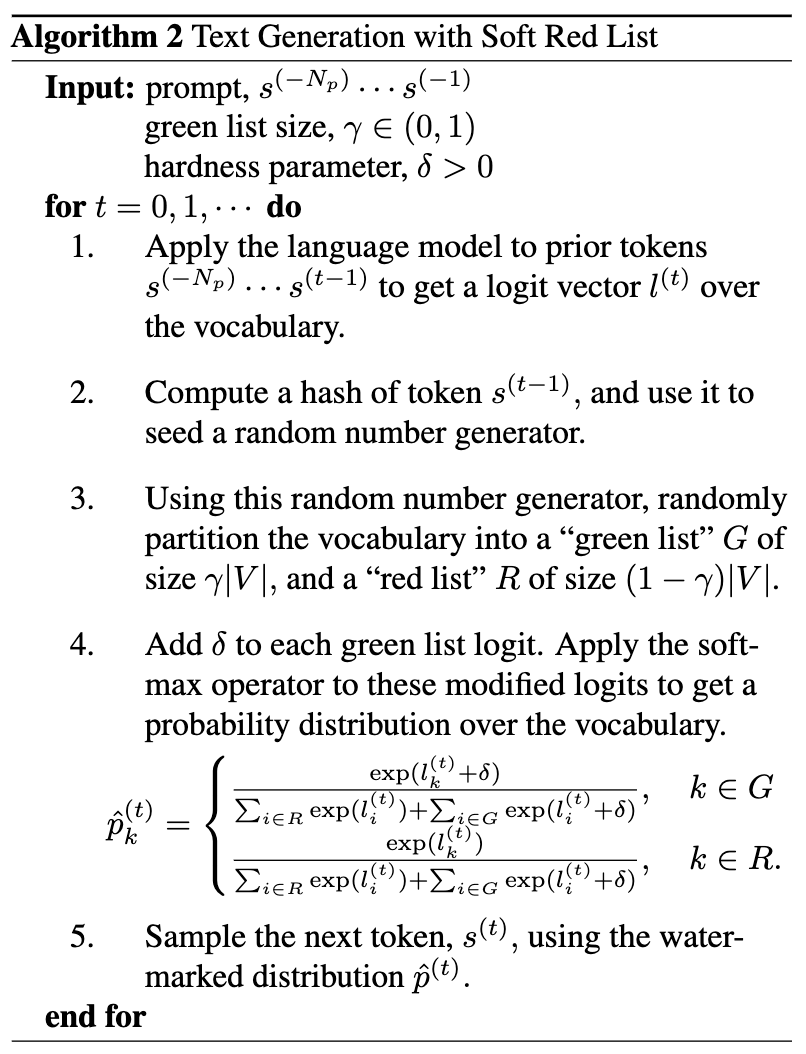
\includegraphics[width=5.5cm]{figure/kirchenbauer2023_algorithm.png}
\end{figure}

\end{vbframe}

% ------------------------------------------------------------------------------
% #38
% ------------------------------------------------------------------------------
\begin{vbframe}{The Watermark Test Statistic}

Let:

\begin{itemize}
    \item \(T\): number of tested tokens,
    \item \(G\): observed number of green tokens,
    \item \(\gamma\): expected green-token fraction under the null.
\end{itemize}

Under the null:

\[
G\sim\mathrm{Binomial}(T,\gamma)
\]

Test statistic:

\[
z=\frac{G-\gamma T}{\sqrt{T\gamma(1-\gamma)}}
\]

\begin{center}
\textbf{The evidence accumulates with text length.}
\end{center}

\citebutton{Kirchenbauer et al., 2023}{https://proceedings.mlr.press/v202/kirchenbauer23a.html}

\end{vbframe}

% ------------------------------------------------------------------------------
% #39
% ------------------------------------------------------------------------------
\begin{vbframe}{Detectability vs Quality}

Increasing the watermark strength \(\delta\) improves detectability but can distort text quality. \citebutton{Kirchenbauer et al., 2023, Fig. 2}{https://proceedings.mlr.press/v202/kirchenbauer23a.html}


\begin{figure}
    \centering
    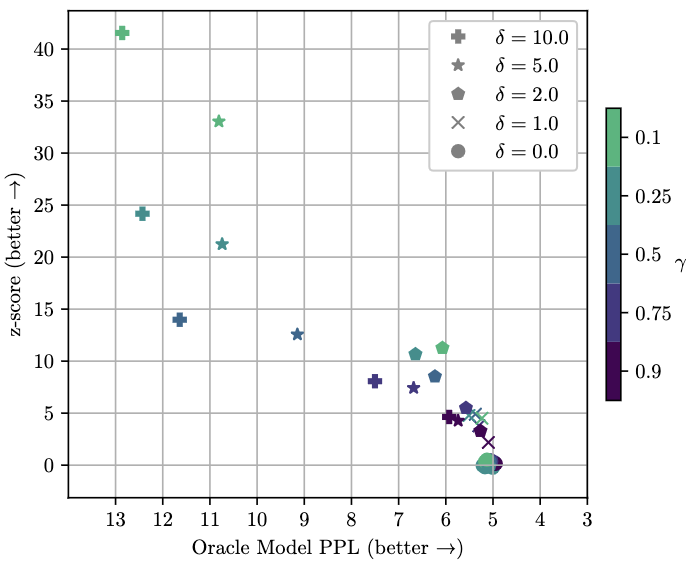
\includegraphics[width=6cm]{figure/kirchenbauer2023_quality_tradeoff_fig2.png}
\end{figure}

%\begin{center}
%\textbf{Watermarking introduces a quality--detectability trade-off.}
%\end{center}

\end{vbframe}

% ------------------------------------------------------------------------------
% #40
% ------------------------------------------------------------------------------
\begin{vbframe}{Do Watermarks Survive Edits?}

\begin{figure}
    \centering
    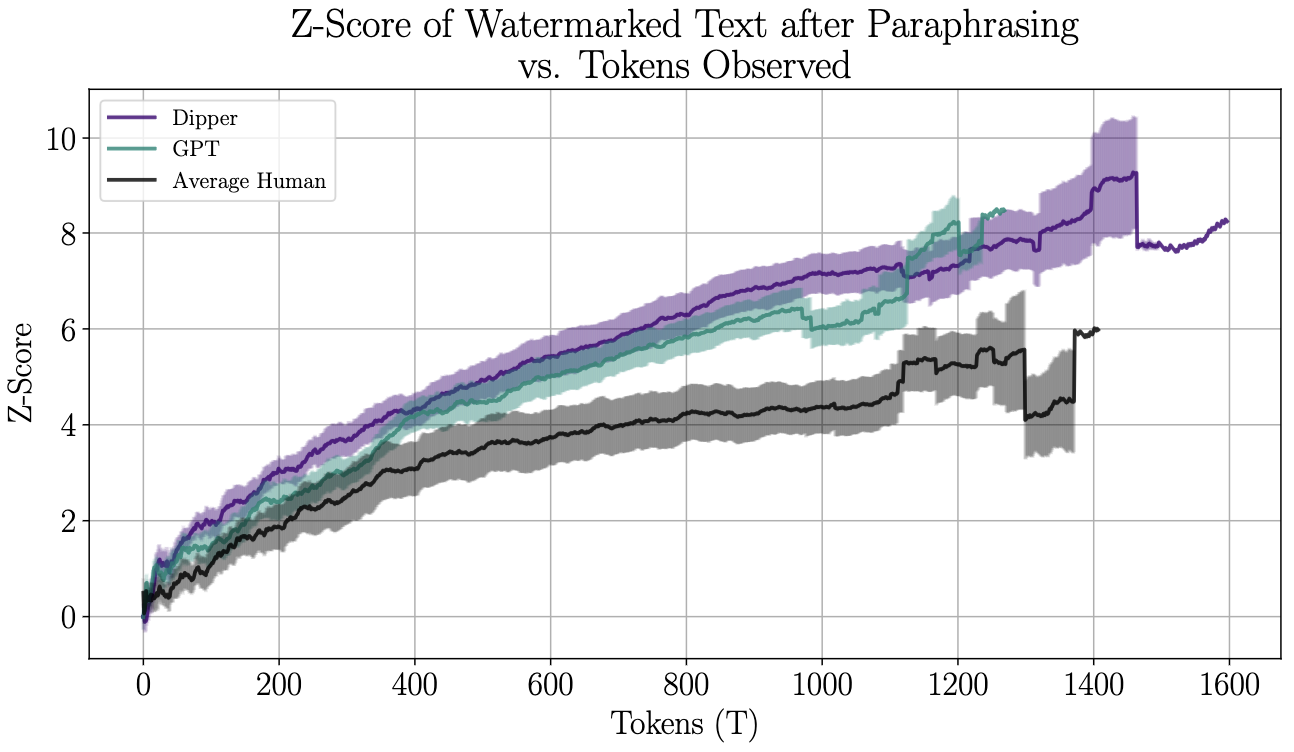
\includegraphics[width=8cm]{figure/kirchenbauer2024_reliability_fig4.png}
\end{figure}

Watermarks can degrade under paraphrasing, rewriting, cropping, and mixing.

But detection can still succeed if enough signal remains.

\citebutton{Kirchenbauer et al., 2024, Fig. 4}{https://arxiv.org/abs/2306.04634}

\end{vbframe}

% ------------------------------------------------------------------------------
% #43
% ------------------------------------------------------------------------------
\begin{vbframe}{SynthID-Text}

SynthID-Text is a keyed generation-time watermark deployed by Google. \citebutton{Dathathri et al., 2024, Nature}
{https://www.nature.com/articles/s41586-024-08025-4}

\begin{figure}
    \centering
    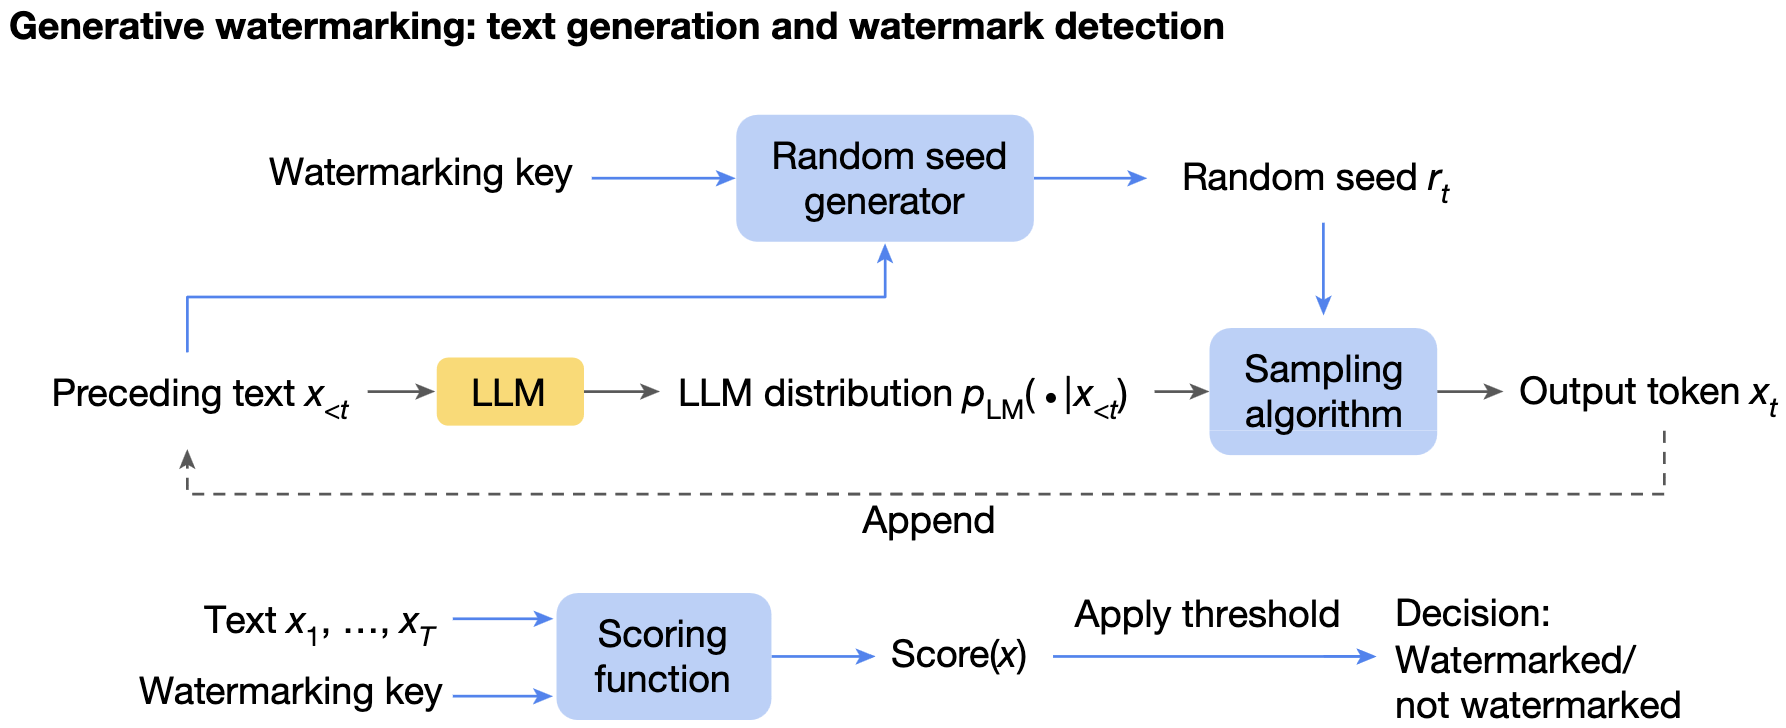
\includegraphics[width=10.8cm]{figure/synthid_text_2024_fig1_overview.png}
\end{figure}

High-level idea:
\[
\text{context} + \text{secret key}
\longrightarrow
\text{modified sampling}
\longrightarrow
\text{detectable statistical signal}
\]


%\begin{itemize}
%    \item no change to model weights
%    \item watermark is inserted during decoding
%    \item detector reconstructs the signal using the secret key
%    \item failure to detect the watermark does \textbf{not} imply human authorship
%\end{itemize}



\end{vbframe}


% ------------------------------------------------------------------------------
% Green lists vs. tournament sampling
% ------------------------------------------------------------------------------

\begin{vbframe}{Green Lists vs.\ Tournament Sampling}
\small
Both methods derive a pseudo-random signal from the
\textbf{secret key + recent context}.

\begin{columns}[T]

\begin{column}{0.48\textwidth}

\textbf{Kirchenbauer et al.}

At each position, split the vocabulary into
\textbf{green} and \textbf{red} tokens.

\[
\hat{\ell}_v =
\begin{cases}
\ell_v+\delta, & v\in G_t\\
\ell_v, & v\notin G_t
\end{cases}
\]

\(\ell_v\): original LM logit for token \(v\)

\begin{itemize}
  \item boost green-token probabilities
  \item detect unusually many green tokens
\end{itemize}

\end{column}

\begin{column}{0.48\textwidth}

\textbf{SynthID-Text}

Generate a keyed pseudo-random signal

\[
r_t=f_r(x_{<t},k)
\]

from context \(x_{<t}\) and secret key \(k\).

\begin{itemize}
  \item sample plausible tokens from the LM
  \item rank them using keyed scores
  \item tournament winner becomes the next token
  \item detect unusually high keyed scores
\end{itemize}

\end{column}

\end{columns}

\end{vbframe}


\begin{vbframe}{SynthID: Tournament Sampling}

\begin{columns}[T]

\begin{column}{0.42\textwidth}

At each position:

\begin{enumerate}
  \item sample several plausible next tokens
  \item score them using the secret key and context
  \item let candidates compete in tournament rounds
  \item output the winner
\end{enumerate}

The watermark changes \textbf{which plausible token is selected},
not which tokens are possible.

\citebutton{Dathathri et al., 2024}
{https://www.nature.com/articles/s41586-024-08025-4}

\end{column}

\begin{column}{0.58\textwidth}

\centering
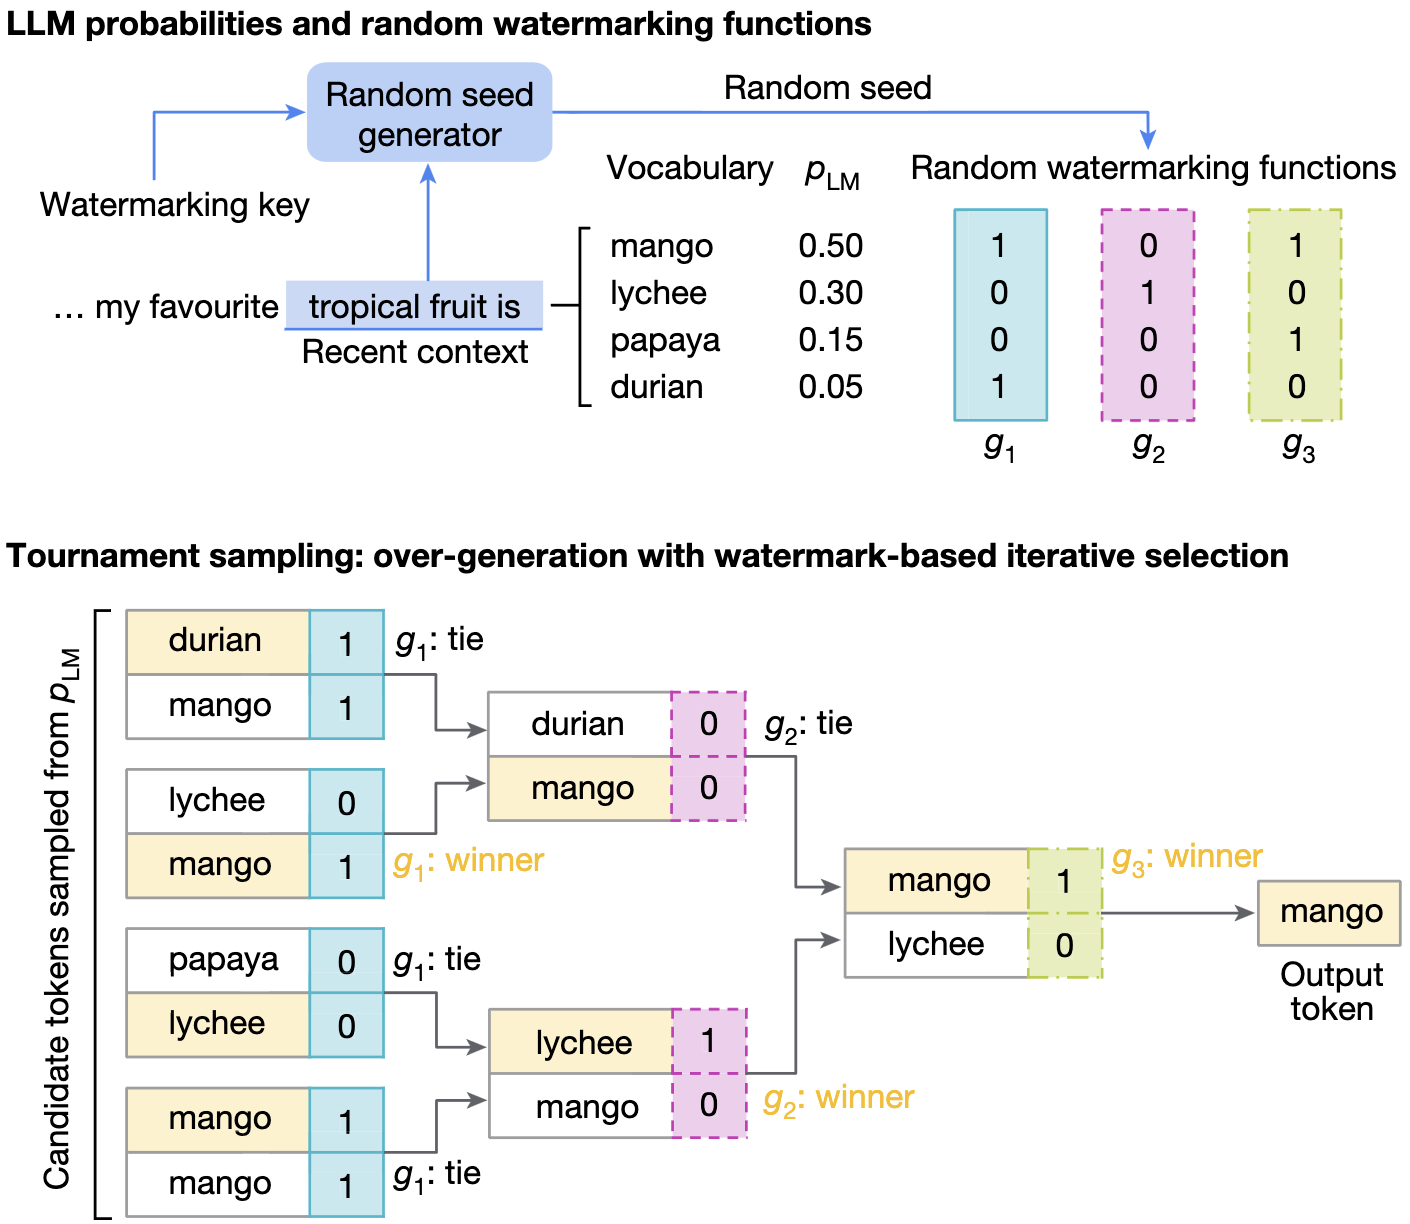
\includegraphics[width=\linewidth]{figure/synthid_fig2_tournament_sampling.png}

\end{column}

\end{columns}

\end{vbframe}


% ------------------------------------------------------------------------------
% SynthID detection
% ------------------------------------------------------------------------------

\begin{vbframe}{SynthID: Detection}

Given the text and secret key, the detector reconstructs the same
pseudo-random signal: $r_t=f_r(x_{<t},k)$

For each token \(x_t\), it computes keyed scores \(g_\ell(x_t,r_t)\).

\[
S(x)=
\frac{1}{mT}
\sum_{t=1}^{T}\sum_{\ell=1}^{m}
g_\ell(x_t,r_t)
\]

\(g_\ell\): keyed score in round \(\ell\); \qquad
\(m\): number of tournament rounds.

Watermarked text should have a systematically higher \(S(x)\) than
ordinary text: $E[S(x)\mid \text{watermarked}]
>
E[S(x)\mid \text{unwatermarked}]$

\begin{itemize}
  \item evidence accumulates over many tokens
  \item detection requires the secret key
  \item the original generating LLM is not required
\end{itemize}

\citebutton{Dathathri et al., 2024}
{https://www.nature.com/articles/s41586-024-08025-4}

\end{vbframe}

\begin{vbframe}{Detectability, Abstention, and Quality}
\small
\begin{figure}
    \centering
    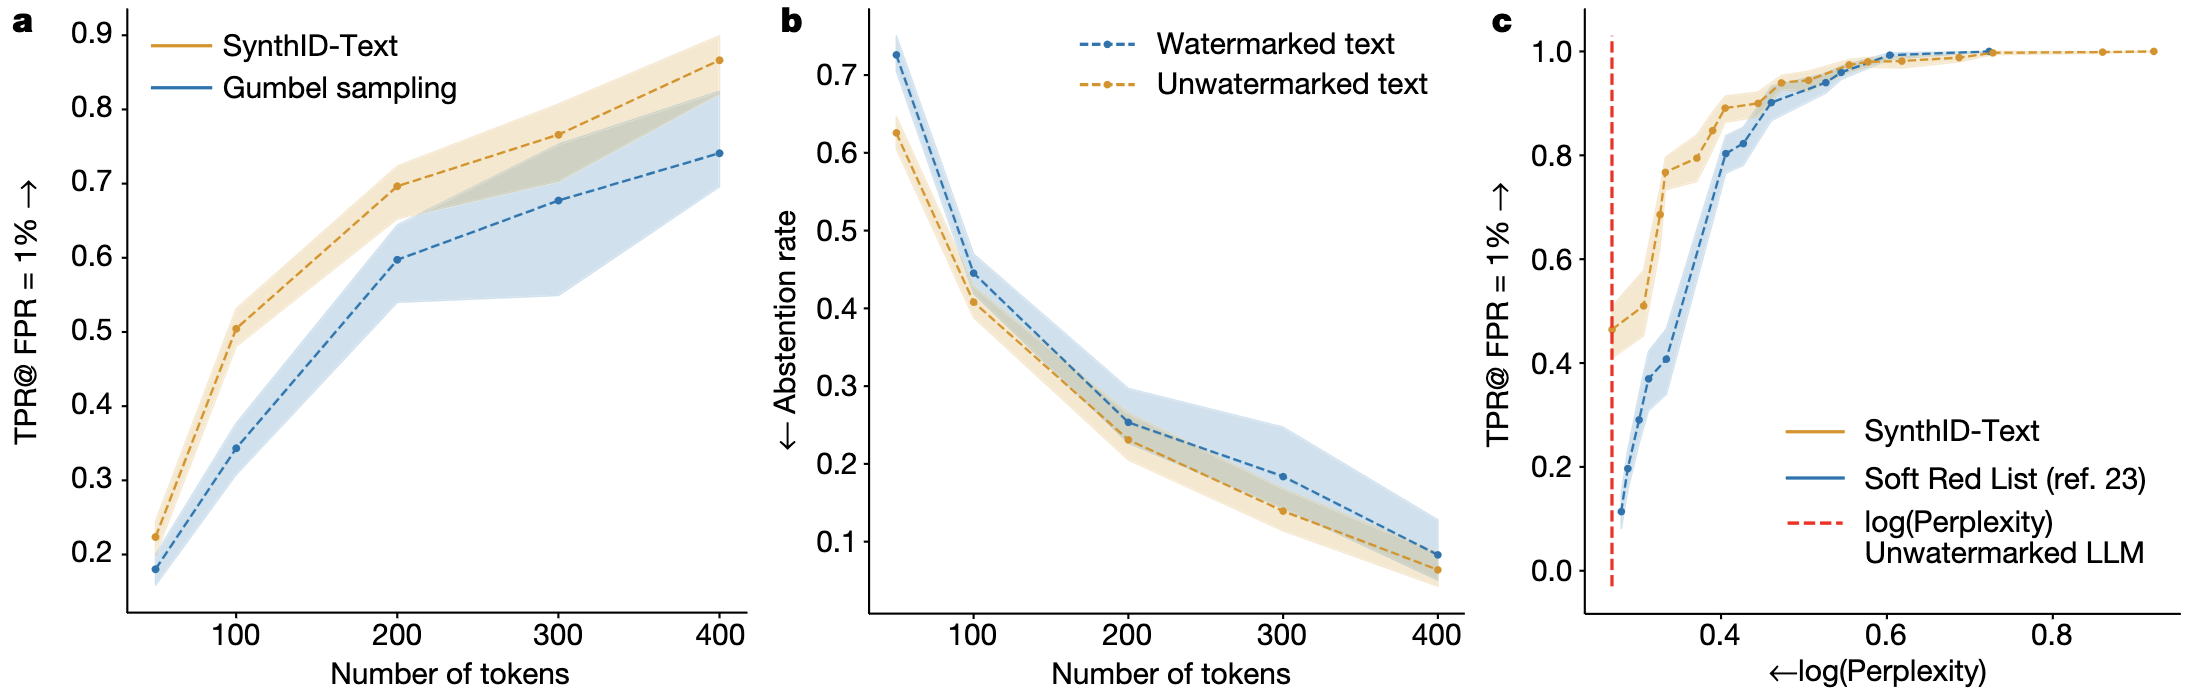
\includegraphics[width=8cm]{figure/synthid_fig3_detectability_abstention_quality.png}
\end{figure}

Key experimental observations:

\begin{itemize}
    \item longer texts provide stronger evidence: 
$T \uparrow \quad \Rightarrow \quad \mathrm{TPR} \uparrow$

    \item selective prediction allows abstention when evidence is weak
    \[
    S(x)<\tau_0: \text{unwatermarked}
    \qquad
    S(x)>\tau_1: \text{watermarked}
    \]

    \item better detection rate than Soft Red List for high-likelihood generations
\end{itemize}
\citebutton{Dathathri et al., 2024, Fig. 3}
{https://www.nature.com/articles/s41586-024-08025-4}

\end{vbframe}


\begin{vbframe}{Quality, Production Deployment, and Limits}

\begin{figure}
    \centering
    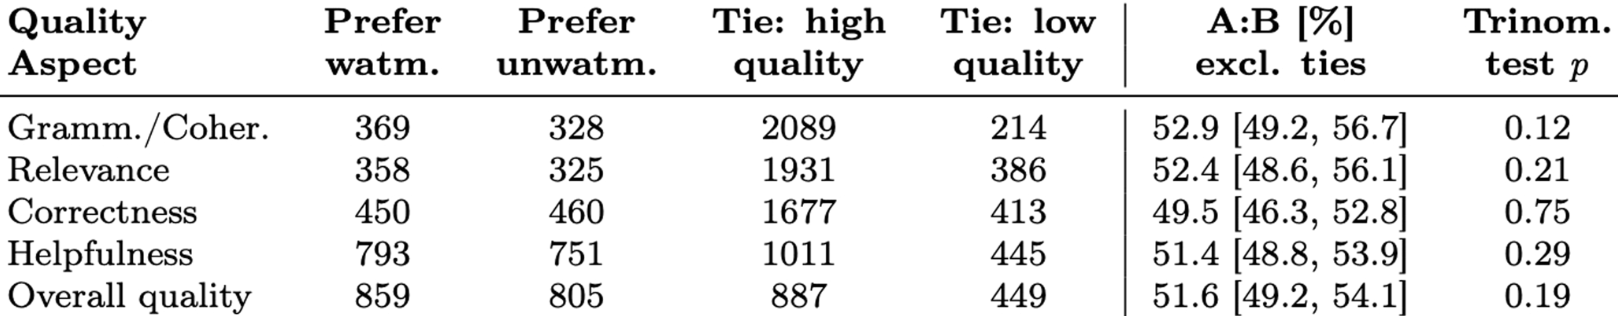
\includegraphics[width=9.8cm]{figure/synthid_ext_table1_human_preferences.png}
\end{figure}

Reported results:

\begin{itemize}
    \item large-scale live experiment on Gemini responses
    \item no statistically significant degradation in thumbs-up/down feedback
    \item human preference study found no significant preference between watermarked and unwatermarked outputs
    \item low reported latency overhead for tournament sampling
\end{itemize}

Important limitations:

\begin{itemize}
    \item short text gives little statistical evidence
    \item low-entropy generation gives little room to encode a watermark
    \item paraphrasing/editing can weaken the signal
    \item watermark detection proves only evidence for a \textbf{specific keyed provenance signal}
\end{itemize}

\citebutton{Dathathri et al., 2024, Extended Data Table 1}
{https://www.nature.com/articles/s41586-024-08025-4}

\end{vbframe}



% ------------------------------------------------------------------------------
% #45
% ------------------------------------------------------------------------------
\begin{vbframe}{Takeaways}

\begin{enumerate}
    \item Passive detectors can be strong in-domain, but their scores depend on distribution, prompt, model, domain, and editing.

    \item Stylometric and likelihood signals are useful, but they are not immutable fingerprints of AI authorship.

    \item Commercial detectors increasingly rely on supervised learning, current training data, hard negatives, and mixed-authorship labels.

    \item Watermarking changes the problem from post-hoc inference to keyed provenance testing.
\end{enumerate}

\end{vbframe}


\endlecture
\end{document}
